% Created by tikzDevice version 0.12 on 2018-10-15 14:40:43
% !TEX encoding = UTF-8 Unicode
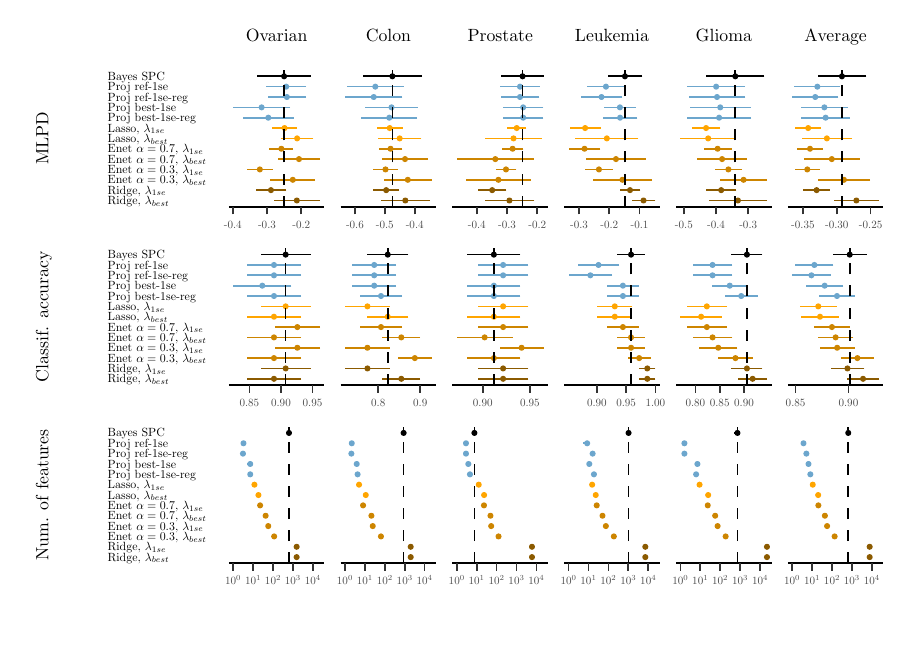
\begin{tikzpicture}[x=1pt,y=1pt]
\definecolor{fillColor}{RGB}{255,255,255}
\path[use as bounding box,fill=fillColor,fill opacity=0.00] (0,0) rectangle (310.76,216.81);
\begin{scope}
\path[clip] (  0.00,204.19) rectangle (  9.66,216.81);
\definecolor{drawColor}{RGB}{255,255,255}
\definecolor{fillColor}{RGB}{255,255,255}

\path[draw=drawColor,line width= 0.6pt,line join=round,line cap=round,fill=fillColor] (  0.00,204.19) rectangle (  9.66,216.81);
\end{scope}
\begin{scope}
\path[clip] (  0.00,139.76) rectangle (  9.66,204.19);
\definecolor{drawColor}{RGB}{255,255,255}
\definecolor{fillColor}{RGB}{255,255,255}

\path[draw=drawColor,line width= 0.6pt,line join=round,line cap=round,fill=fillColor] (  0.00,139.76) rectangle (  9.66,204.19);
\end{scope}
\begin{scope}
\path[clip] (  0.00, 75.32) rectangle (  9.66,139.76);
\definecolor{drawColor}{RGB}{255,255,255}
\definecolor{fillColor}{RGB}{255,255,255}

\path[draw=drawColor,line width= 0.6pt,line join=round,line cap=round,fill=fillColor] (  0.00, 75.32) rectangle (  9.66,139.76);
\end{scope}
\begin{scope}
\path[clip] (  0.00,  0.00) rectangle (  9.66, 75.32);
\definecolor{drawColor}{RGB}{255,255,255}
\definecolor{fillColor}{RGB}{255,255,255}

\path[draw=drawColor,line width= 0.6pt,line join=round,line cap=round,fill=fillColor] (  0.00,  0.00) rectangle (  9.66, 75.32);
\end{scope}
\begin{scope}
\path[clip] (  9.66,204.19) rectangle ( 68.38,216.81);
\definecolor{drawColor}{RGB}{255,255,255}
\definecolor{fillColor}{RGB}{255,255,255}

\path[draw=drawColor,line width= 0.6pt,line join=round,line cap=round,fill=fillColor] (  9.66,204.19) rectangle ( 68.38,216.81);
\end{scope}
\begin{scope}
\path[clip] (  9.66,139.76) rectangle ( 68.38,204.19);
\definecolor{drawColor}{RGB}{255,255,255}
\definecolor{fillColor}{RGB}{255,255,255}

\path[draw=drawColor,line width= 0.6pt,line join=round,line cap=round,fill=fillColor] (  9.66,139.76) rectangle ( 68.38,204.19);
\end{scope}
\begin{scope}
\path[clip] (  9.66, 75.32) rectangle ( 68.38,139.76);
\definecolor{drawColor}{RGB}{255,255,255}
\definecolor{fillColor}{RGB}{255,255,255}

\path[draw=drawColor,line width= 0.6pt,line join=round,line cap=round,fill=fillColor] (  9.66, 75.32) rectangle ( 68.38,139.76);
\end{scope}
\begin{scope}
\path[clip] (  9.66,  0.00) rectangle ( 68.38, 75.32);
\definecolor{drawColor}{RGB}{255,255,255}
\definecolor{fillColor}{RGB}{255,255,255}

\path[draw=drawColor,line width= 0.6pt,line join=round,line cap=round,fill=fillColor] (  9.66,  0.00) rectangle ( 68.38, 75.32);
\end{scope}
\begin{scope}
\path[clip] ( 68.38,204.19) rectangle (108.78,216.81);
\definecolor{drawColor}{RGB}{255,255,255}
\definecolor{fillColor}{RGB}{255,255,255}

\path[draw=drawColor,line width= 0.6pt,line join=round,line cap=round,fill=fillColor] ( 68.38,204.19) rectangle (108.78,216.81);
\end{scope}
\begin{scope}
\path[clip] ( 68.38,139.76) rectangle (108.78,204.19);
\definecolor{drawColor}{RGB}{255,255,255}
\definecolor{fillColor}{RGB}{255,255,255}

\path[draw=drawColor,line width= 0.6pt,line join=round,line cap=round,fill=fillColor] ( 68.38,139.76) rectangle (108.78,204.19);
\end{scope}
\begin{scope}
\path[clip] ( 68.38, 75.32) rectangle (108.78,139.76);
\definecolor{drawColor}{RGB}{255,255,255}
\definecolor{fillColor}{RGB}{255,255,255}

\path[draw=drawColor,line width= 0.6pt,line join=round,line cap=round,fill=fillColor] ( 68.38, 75.32) rectangle (108.78,139.76);
\end{scope}
\begin{scope}
\path[clip] ( 68.38,  0.00) rectangle (108.78, 75.32);
\definecolor{drawColor}{RGB}{255,255,255}
\definecolor{fillColor}{RGB}{255,255,255}

\path[draw=drawColor,line width= 0.6pt,line join=round,line cap=round,fill=fillColor] ( 68.38,  0.00) rectangle (108.78, 75.32);
\end{scope}
\begin{scope}
\path[clip] (108.78,204.19) rectangle (149.17,216.81);
\definecolor{drawColor}{RGB}{255,255,255}
\definecolor{fillColor}{RGB}{255,255,255}

\path[draw=drawColor,line width= 0.6pt,line join=round,line cap=round,fill=fillColor] (108.78,204.19) rectangle (149.17,216.81);
\end{scope}
\begin{scope}
\path[clip] (108.78,139.76) rectangle (149.17,204.19);
\definecolor{drawColor}{RGB}{255,255,255}
\definecolor{fillColor}{RGB}{255,255,255}

\path[draw=drawColor,line width= 0.6pt,line join=round,line cap=round,fill=fillColor] (108.78,139.76) rectangle (149.17,204.19);
\end{scope}
\begin{scope}
\path[clip] (108.78, 75.32) rectangle (149.17,139.76);
\definecolor{drawColor}{RGB}{255,255,255}
\definecolor{fillColor}{RGB}{255,255,255}

\path[draw=drawColor,line width= 0.6pt,line join=round,line cap=round,fill=fillColor] (108.78, 75.32) rectangle (149.17,139.76);
\end{scope}
\begin{scope}
\path[clip] (108.78,  0.00) rectangle (149.17, 75.32);
\definecolor{drawColor}{RGB}{255,255,255}
\definecolor{fillColor}{RGB}{255,255,255}

\path[draw=drawColor,line width= 0.6pt,line join=round,line cap=round,fill=fillColor] (108.78,  0.00) rectangle (149.17, 75.32);
\end{scope}
\begin{scope}
\path[clip] (149.17,204.19) rectangle (189.57,216.81);
\definecolor{drawColor}{RGB}{255,255,255}
\definecolor{fillColor}{RGB}{255,255,255}

\path[draw=drawColor,line width= 0.6pt,line join=round,line cap=round,fill=fillColor] (149.17,204.19) rectangle (189.57,216.81);
\end{scope}
\begin{scope}
\path[clip] (149.17,139.76) rectangle (189.57,204.19);
\definecolor{drawColor}{RGB}{255,255,255}
\definecolor{fillColor}{RGB}{255,255,255}

\path[draw=drawColor,line width= 0.6pt,line join=round,line cap=round,fill=fillColor] (149.17,139.76) rectangle (189.57,204.19);
\end{scope}
\begin{scope}
\path[clip] (149.17, 75.32) rectangle (189.57,139.76);
\definecolor{drawColor}{RGB}{255,255,255}
\definecolor{fillColor}{RGB}{255,255,255}

\path[draw=drawColor,line width= 0.6pt,line join=round,line cap=round,fill=fillColor] (149.17, 75.32) rectangle (189.57,139.76);
\end{scope}
\begin{scope}
\path[clip] (149.17,  0.00) rectangle (189.57, 75.32);
\definecolor{drawColor}{RGB}{255,255,255}
\definecolor{fillColor}{RGB}{255,255,255}

\path[draw=drawColor,line width= 0.6pt,line join=round,line cap=round,fill=fillColor] (149.17,  0.00) rectangle (189.57, 75.32);
\end{scope}
\begin{scope}
\path[clip] (189.57,204.19) rectangle (229.97,216.81);
\definecolor{drawColor}{RGB}{255,255,255}
\definecolor{fillColor}{RGB}{255,255,255}

\path[draw=drawColor,line width= 0.6pt,line join=round,line cap=round,fill=fillColor] (189.57,204.19) rectangle (229.97,216.81);
\end{scope}
\begin{scope}
\path[clip] (189.57,139.76) rectangle (229.97,204.19);
\definecolor{drawColor}{RGB}{255,255,255}
\definecolor{fillColor}{RGB}{255,255,255}

\path[draw=drawColor,line width= 0.6pt,line join=round,line cap=round,fill=fillColor] (189.57,139.76) rectangle (229.97,204.19);
\end{scope}
\begin{scope}
\path[clip] (189.57, 75.32) rectangle (229.97,139.76);
\definecolor{drawColor}{RGB}{255,255,255}
\definecolor{fillColor}{RGB}{255,255,255}

\path[draw=drawColor,line width= 0.6pt,line join=round,line cap=round,fill=fillColor] (189.57, 75.32) rectangle (229.97,139.76);
\end{scope}
\begin{scope}
\path[clip] (189.57,  0.00) rectangle (229.97, 75.32);
\definecolor{drawColor}{RGB}{255,255,255}
\definecolor{fillColor}{RGB}{255,255,255}

\path[draw=drawColor,line width= 0.6pt,line join=round,line cap=round,fill=fillColor] (189.57,  0.00) rectangle (229.97, 75.32);
\end{scope}
\begin{scope}
\path[clip] (229.97,204.19) rectangle (270.36,216.81);
\definecolor{drawColor}{RGB}{255,255,255}
\definecolor{fillColor}{RGB}{255,255,255}

\path[draw=drawColor,line width= 0.6pt,line join=round,line cap=round,fill=fillColor] (229.97,204.19) rectangle (270.36,216.81);
\end{scope}
\begin{scope}
\path[clip] (229.97,139.76) rectangle (270.36,204.19);
\definecolor{drawColor}{RGB}{255,255,255}
\definecolor{fillColor}{RGB}{255,255,255}

\path[draw=drawColor,line width= 0.6pt,line join=round,line cap=round,fill=fillColor] (229.97,139.76) rectangle (270.36,204.19);
\end{scope}
\begin{scope}
\path[clip] (229.97, 75.32) rectangle (270.36,139.76);
\definecolor{drawColor}{RGB}{255,255,255}
\definecolor{fillColor}{RGB}{255,255,255}

\path[draw=drawColor,line width= 0.6pt,line join=round,line cap=round,fill=fillColor] (229.97, 75.32) rectangle (270.36,139.76);
\end{scope}
\begin{scope}
\path[clip] (229.97,  0.00) rectangle (270.36, 75.32);
\definecolor{drawColor}{RGB}{255,255,255}
\definecolor{fillColor}{RGB}{255,255,255}

\path[draw=drawColor,line width= 0.6pt,line join=round,line cap=round,fill=fillColor] (229.97,  0.00) rectangle (270.36, 75.32);
\end{scope}
\begin{scope}
\path[clip] (270.36,204.19) rectangle (310.76,216.81);
\definecolor{drawColor}{RGB}{255,255,255}
\definecolor{fillColor}{RGB}{255,255,255}

\path[draw=drawColor,line width= 0.6pt,line join=round,line cap=round,fill=fillColor] (270.36,204.19) rectangle (310.76,216.81);
\end{scope}
\begin{scope}
\path[clip] (270.36,139.76) rectangle (310.76,204.19);
\definecolor{drawColor}{RGB}{255,255,255}
\definecolor{fillColor}{RGB}{255,255,255}

\path[draw=drawColor,line width= 0.6pt,line join=round,line cap=round,fill=fillColor] (270.36,139.76) rectangle (310.76,204.19);
\end{scope}
\begin{scope}
\path[clip] (270.36, 75.32) rectangle (310.76,139.76);
\definecolor{drawColor}{RGB}{255,255,255}
\definecolor{fillColor}{RGB}{255,255,255}

\path[draw=drawColor,line width= 0.6pt,line join=round,line cap=round,fill=fillColor] (270.36, 75.32) rectangle (310.76,139.76);
\end{scope}
\begin{scope}
\path[clip] (270.36,  0.00) rectangle (310.76, 75.32);
\definecolor{drawColor}{RGB}{255,255,255}
\definecolor{fillColor}{RGB}{255,255,255}

\path[draw=drawColor,line width= 0.6pt,line join=round,line cap=round,fill=fillColor] (270.36,  0.00) rectangle (310.76, 75.32);
\end{scope}
\begin{scope}
\path[clip] (  2.75,206.94) rectangle (  9.66,216.81);
\definecolor{fillColor}{RGB}{255,255,255}

\path[fill=fillColor] (  2.75,206.94) rectangle (  9.66,216.81);
\end{scope}
\begin{scope}
\path[clip] (  2.75,152.11) rectangle (  9.66,201.48);
\definecolor{drawColor}{RGB}{0,0,0}

\node[text=drawColor,rotate= 90.00,anchor=base,inner sep=0pt, outer sep=0pt, scale=  0.64] at (  7.47,176.80) {MLPD};
\end{scope}
\begin{scope}
\path[clip] (  2.75, 87.68) rectangle (  9.66,137.05);
\definecolor{drawColor}{RGB}{0,0,0}

\node[text=drawColor,rotate= 90.00,anchor=base,inner sep=0pt, outer sep=0pt, scale=  0.64] at (  7.47,112.36) {Classif. accuracy};
\end{scope}
\begin{scope}
\path[clip] (  2.75, 23.25) rectangle (  9.66, 72.61);
\definecolor{drawColor}{RGB}{0,0,0}

\node[text=drawColor,rotate= 90.00,anchor=base,inner sep=0pt, outer sep=0pt, scale=  0.64] at (  7.47, 47.93) {Num. of features};
\end{scope}
\begin{scope}
\path[clip] ( 27.10,152.11) rectangle ( 66.82,201.48);
\definecolor{drawColor}{RGB}{0,0,0}

\node[text=drawColor,anchor=base west,inner sep=0pt, outer sep=0pt, scale=  0.43] at ( 28.91,197.76) {Bayes SPC};

\node[text=drawColor,anchor=base west,inner sep=0pt, outer sep=0pt, scale=  0.43] at ( 28.91,194.02) {Proj ref-1se};

\node[text=drawColor,anchor=base west,inner sep=0pt, outer sep=0pt, scale=  0.43] at ( 28.91,190.28) {Proj ref-1se-reg};

\node[text=drawColor,anchor=base west,inner sep=0pt, outer sep=0pt, scale=  0.43] at ( 28.91,186.55) {Proj best-1se};

\node[text=drawColor,anchor=base west,inner sep=0pt, outer sep=0pt, scale=  0.43] at ( 28.91,182.81) {Proj best-1se-reg};

\node[text=drawColor,anchor=base west,inner sep=0pt, outer sep=0pt, scale=  0.43] at ( 28.91,179.07) {Lasso, $\lambda_\text{1se}$};

\node[text=drawColor,anchor=base west,inner sep=0pt, outer sep=0pt, scale=  0.43] at ( 28.91,175.33) {Lasso, $\lambda_\text{best}$};

\node[text=drawColor,anchor=base west,inner sep=0pt, outer sep=0pt, scale=  0.43] at ( 28.91,171.59) {Enet $\alpha=0.7$, $\lambda_\text{1se}$};

\node[text=drawColor,anchor=base west,inner sep=0pt, outer sep=0pt, scale=  0.43] at ( 28.91,167.85) {Enet $\alpha=0.7$, $\lambda_\text{best}$};

\node[text=drawColor,anchor=base west,inner sep=0pt, outer sep=0pt, scale=  0.43] at ( 28.91,164.11) {Enet $\alpha=0.3$, $\lambda_\text{1se}$};

\node[text=drawColor,anchor=base west,inner sep=0pt, outer sep=0pt, scale=  0.43] at ( 28.91,160.37) {Enet $\alpha=0.3$, $\lambda_\text{best}$};

\node[text=drawColor,anchor=base west,inner sep=0pt, outer sep=0pt, scale=  0.43] at ( 28.91,156.63) {Ridge, $\lambda_\text{1se}$};

\node[text=drawColor,anchor=base west,inner sep=0pt, outer sep=0pt, scale=  0.43] at ( 28.91,152.89) {Ridge, $\lambda_\text{best}$};
\end{scope}
\begin{scope}
\path[clip] ( 27.10, 87.68) rectangle ( 66.82,137.05);
\definecolor{drawColor}{RGB}{0,0,0}

\node[text=drawColor,anchor=base west,inner sep=0pt, outer sep=0pt, scale=  0.43] at ( 28.91,133.33) {Bayes SPC};

\node[text=drawColor,anchor=base west,inner sep=0pt, outer sep=0pt, scale=  0.43] at ( 28.91,129.59) {Proj ref-1se};

\node[text=drawColor,anchor=base west,inner sep=0pt, outer sep=0pt, scale=  0.43] at ( 28.91,125.85) {Proj ref-1se-reg};

\node[text=drawColor,anchor=base west,inner sep=0pt, outer sep=0pt, scale=  0.43] at ( 28.91,122.11) {Proj best-1se};

\node[text=drawColor,anchor=base west,inner sep=0pt, outer sep=0pt, scale=  0.43] at ( 28.91,118.37) {Proj best-1se-reg};

\node[text=drawColor,anchor=base west,inner sep=0pt, outer sep=0pt, scale=  0.43] at ( 28.91,114.63) {Lasso, $\lambda_\text{1se}$};

\node[text=drawColor,anchor=base west,inner sep=0pt, outer sep=0pt, scale=  0.43] at ( 28.91,110.89) {Lasso, $\lambda_\text{best}$};

\node[text=drawColor,anchor=base west,inner sep=0pt, outer sep=0pt, scale=  0.43] at ( 28.91,107.16) {Enet $\alpha=0.7$, $\lambda_\text{1se}$};

\node[text=drawColor,anchor=base west,inner sep=0pt, outer sep=0pt, scale=  0.43] at ( 28.91,103.42) {Enet $\alpha=0.7$, $\lambda_\text{best}$};

\node[text=drawColor,anchor=base west,inner sep=0pt, outer sep=0pt, scale=  0.43] at ( 28.91, 99.68) {Enet $\alpha=0.3$, $\lambda_\text{1se}$};

\node[text=drawColor,anchor=base west,inner sep=0pt, outer sep=0pt, scale=  0.43] at ( 28.91, 95.94) {Enet $\alpha=0.3$, $\lambda_\text{best}$};

\node[text=drawColor,anchor=base west,inner sep=0pt, outer sep=0pt, scale=  0.43] at ( 28.91, 92.20) {Ridge, $\lambda_\text{1se}$};

\node[text=drawColor,anchor=base west,inner sep=0pt, outer sep=0pt, scale=  0.43] at ( 28.91, 88.46) {Ridge, $\lambda_\text{best}$};
\end{scope}
\begin{scope}
\path[clip] ( 27.10, 23.25) rectangle ( 66.82, 72.61);
\definecolor{drawColor}{RGB}{0,0,0}

\node[text=drawColor,anchor=base west,inner sep=0pt, outer sep=0pt, scale=  0.43] at ( 28.91, 68.90) {Bayes SPC};

\node[text=drawColor,anchor=base west,inner sep=0pt, outer sep=0pt, scale=  0.43] at ( 28.91, 65.16) {Proj ref-1se};

\node[text=drawColor,anchor=base west,inner sep=0pt, outer sep=0pt, scale=  0.43] at ( 28.91, 61.42) {Proj ref-1se-reg};

\node[text=drawColor,anchor=base west,inner sep=0pt, outer sep=0pt, scale=  0.43] at ( 28.91, 57.68) {Proj best-1se};

\node[text=drawColor,anchor=base west,inner sep=0pt, outer sep=0pt, scale=  0.43] at ( 28.91, 53.94) {Proj best-1se-reg};

\node[text=drawColor,anchor=base west,inner sep=0pt, outer sep=0pt, scale=  0.43] at ( 28.91, 50.20) {Lasso, $\lambda_\text{1se}$};

\node[text=drawColor,anchor=base west,inner sep=0pt, outer sep=0pt, scale=  0.43] at ( 28.91, 46.46) {Lasso, $\lambda_\text{best}$};

\node[text=drawColor,anchor=base west,inner sep=0pt, outer sep=0pt, scale=  0.43] at ( 28.91, 42.72) {Enet $\alpha=0.7$, $\lambda_\text{1se}$};

\node[text=drawColor,anchor=base west,inner sep=0pt, outer sep=0pt, scale=  0.43] at ( 28.91, 38.98) {Enet $\alpha=0.7$, $\lambda_\text{best}$};

\node[text=drawColor,anchor=base west,inner sep=0pt, outer sep=0pt, scale=  0.43] at ( 28.91, 35.24) {Enet $\alpha=0.3$, $\lambda_\text{1se}$};

\node[text=drawColor,anchor=base west,inner sep=0pt, outer sep=0pt, scale=  0.43] at ( 28.91, 31.50) {Enet $\alpha=0.3$, $\lambda_\text{best}$};

\node[text=drawColor,anchor=base west,inner sep=0pt, outer sep=0pt, scale=  0.43] at ( 28.91, 27.76) {Ridge, $\lambda_\text{1se}$};

\node[text=drawColor,anchor=base west,inner sep=0pt, outer sep=0pt, scale=  0.43] at ( 28.91, 24.03) {Ridge, $\lambda_\text{best}$};
\end{scope}
\begin{scope}
\path[clip] ( 72.68,206.94) rectangle (107.22,216.81);
\definecolor{drawColor}{RGB}{0,0,0}

\node[text=drawColor,anchor=base,inner sep=0pt, outer sep=0pt, scale=  0.64] at ( 89.95,211.95) {Ovarian};
\end{scope}
\begin{scope}
\path[clip] ( 72.68,152.11) rectangle (107.22,201.48);
\definecolor{fillColor}{RGB}{255,255,255}

\path[fill=fillColor] ( 72.68,152.11) rectangle (107.22,201.48);
\definecolor{drawColor}{RGB}{0,0,0}
\definecolor{fillColor}{RGB}{0,0,0}

\path[draw=drawColor,line width= 0.4pt,line join=round,line cap=round,fill=fillColor] ( 92.65,199.23) circle (  0.89);
\definecolor{drawColor}{RGB}{108,166,205}
\definecolor{fillColor}{RGB}{108,166,205}

\path[draw=drawColor,line width= 0.4pt,line join=round,line cap=round,fill=fillColor] ( 93.41,195.49) circle (  0.89);

\path[draw=drawColor,line width= 0.4pt,line join=round,line cap=round,fill=fillColor] ( 93.66,191.75) circle (  0.89);

\path[draw=drawColor,line width= 0.4pt,line join=round,line cap=round,fill=fillColor] ( 84.53,188.01) circle (  0.89);

\path[draw=drawColor,line width= 0.4pt,line join=round,line cap=round,fill=fillColor] ( 86.95,184.28) circle (  0.89);
\definecolor{drawColor}{RGB}{255,165,0}
\definecolor{fillColor}{RGB}{255,165,0}

\path[draw=drawColor,line width= 0.4pt,line join=round,line cap=round,fill=fillColor] ( 92.82,180.54) circle (  0.89);

\path[draw=drawColor,line width= 0.4pt,line join=round,line cap=round,fill=fillColor] ( 97.36,176.80) circle (  0.89);
\definecolor{drawColor}{RGB}{205,133,0}
\definecolor{fillColor}{RGB}{205,133,0}

\path[draw=drawColor,line width= 0.4pt,line join=round,line cap=round,fill=fillColor] ( 91.67,173.06) circle (  0.89);

\path[draw=drawColor,line width= 0.4pt,line join=round,line cap=round,fill=fillColor] ( 98.04,169.32) circle (  0.89);

\path[draw=drawColor,line width= 0.4pt,line join=round,line cap=round,fill=fillColor] ( 83.89,165.58) circle (  0.89);

\path[draw=drawColor,line width= 0.4pt,line join=round,line cap=round,fill=fillColor] ( 95.80,161.84) circle (  0.89);
\definecolor{drawColor}{RGB}{139,90,0}
\definecolor{fillColor}{RGB}{139,90,0}

\path[draw=drawColor,line width= 0.4pt,line join=round,line cap=round,fill=fillColor] ( 87.91,158.10) circle (  0.89);

\path[draw=drawColor,line width= 0.4pt,line join=round,line cap=round,fill=fillColor] ( 97.26,154.36) circle (  0.89);
\definecolor{drawColor}{RGB}{0,0,0}

\path[draw=drawColor,line width= 0.6pt,line join=round] (102.28,199.23) --
	(102.28,199.23);

\path[draw=drawColor,line width= 0.6pt,line join=round] (102.28,199.23) --
	( 83.02,199.23);

\path[draw=drawColor,line width= 0.6pt,line join=round] ( 83.02,199.23) --
	( 83.02,199.23);
\definecolor{drawColor}{RGB}{108,166,205}

\path[draw=drawColor,line width= 0.6pt,line join=round] (100.62,195.49) --
	(100.62,195.49);

\path[draw=drawColor,line width= 0.6pt,line join=round] (100.62,195.49) --
	( 86.20,195.49);

\path[draw=drawColor,line width= 0.6pt,line join=round] ( 86.20,195.49) --
	( 86.20,195.49);

\path[draw=drawColor,line width= 0.6pt,line join=round] (100.64,191.75) --
	(100.64,191.75);

\path[draw=drawColor,line width= 0.6pt,line join=round] (100.64,191.75) --
	( 86.67,191.75);

\path[draw=drawColor,line width= 0.6pt,line join=round] ( 86.67,191.75) --
	( 86.67,191.75);

\path[draw=drawColor,line width= 0.6pt,line join=round] ( 94.82,188.01) --
	( 94.82,188.01);

\path[draw=drawColor,line width= 0.6pt,line join=round] ( 94.82,188.01) --
	( 74.25,188.01);

\path[draw=drawColor,line width= 0.6pt,line join=round] ( 74.25,188.01) --
	( 74.25,188.01);

\path[draw=drawColor,line width= 0.6pt,line join=round] ( 96.08,184.28) --
	( 96.08,184.28);

\path[draw=drawColor,line width= 0.6pt,line join=round] ( 96.08,184.28) --
	( 77.82,184.28);

\path[draw=drawColor,line width= 0.6pt,line join=round] ( 77.82,184.28) --
	( 77.82,184.28);
\definecolor{drawColor}{RGB}{255,165,0}

\path[draw=drawColor,line width= 0.6pt,line join=round] ( 97.36,180.54) --
	( 97.36,180.54);

\path[draw=drawColor,line width= 0.6pt,line join=round] ( 97.36,180.54) --
	( 88.28,180.54);

\path[draw=drawColor,line width= 0.6pt,line join=round] ( 88.28,180.54) --
	( 88.28,180.54);

\path[draw=drawColor,line width= 0.6pt,line join=round] (103.21,176.80) --
	(103.21,176.80);

\path[draw=drawColor,line width= 0.6pt,line join=round] (103.21,176.80) --
	( 91.51,176.80);

\path[draw=drawColor,line width= 0.6pt,line join=round] ( 91.51,176.80) --
	( 91.51,176.80);
\definecolor{drawColor}{RGB}{205,133,0}

\path[draw=drawColor,line width= 0.6pt,line join=round] ( 95.96,173.06) --
	( 95.96,173.06);

\path[draw=drawColor,line width= 0.6pt,line join=round] ( 95.96,173.06) --
	( 87.38,173.06);

\path[draw=drawColor,line width= 0.6pt,line join=round] ( 87.38,173.06) --
	( 87.38,173.06);

\path[draw=drawColor,line width= 0.6pt,line join=round] (105.65,169.32) --
	(105.65,169.32);

\path[draw=drawColor,line width= 0.6pt,line join=round] (105.65,169.32) --
	( 90.44,169.32);

\path[draw=drawColor,line width= 0.6pt,line join=round] ( 90.44,169.32) --
	( 90.44,169.32);

\path[draw=drawColor,line width= 0.6pt,line join=round] ( 88.59,165.58) --
	( 88.59,165.58);

\path[draw=drawColor,line width= 0.6pt,line join=round] ( 88.59,165.58) --
	( 79.19,165.58);

\path[draw=drawColor,line width= 0.6pt,line join=round] ( 79.19,165.58) --
	( 79.19,165.58);

\path[draw=drawColor,line width= 0.6pt,line join=round] (103.89,161.84) --
	(103.89,161.84);

\path[draw=drawColor,line width= 0.6pt,line join=round] (103.89,161.84) --
	( 87.72,161.84);

\path[draw=drawColor,line width= 0.6pt,line join=round] ( 87.72,161.84) --
	( 87.72,161.84);
\definecolor{drawColor}{RGB}{139,90,0}

\path[draw=drawColor,line width= 0.6pt,line join=round] ( 93.48,158.10) --
	( 93.48,158.10);

\path[draw=drawColor,line width= 0.6pt,line join=round] ( 93.48,158.10) --
	( 82.34,158.10);

\path[draw=drawColor,line width= 0.6pt,line join=round] ( 82.34,158.10) --
	( 82.34,158.10);

\path[draw=drawColor,line width= 0.6pt,line join=round] (105.59,154.36) --
	(105.59,154.36);

\path[draw=drawColor,line width= 0.6pt,line join=round] (105.59,154.36) --
	( 88.94,154.36);

\path[draw=drawColor,line width= 0.6pt,line join=round] ( 88.94,154.36) --
	( 88.94,154.36);
\definecolor{drawColor}{RGB}{0,0,0}

\path[draw=drawColor,line width= 0.6pt,dash pattern=on 4pt off 4pt ,line join=round] ( 92.65,152.11) -- ( 92.65,201.48);
\end{scope}
\begin{scope}
\path[clip] ( 72.68, 87.68) rectangle (107.22,137.05);
\definecolor{fillColor}{RGB}{255,255,255}

\path[fill=fillColor] ( 72.68, 87.68) rectangle (107.22,137.05);
\definecolor{drawColor}{RGB}{0,0,0}
\definecolor{fillColor}{RGB}{0,0,0}

\path[draw=drawColor,line width= 0.4pt,line join=round,line cap=round,fill=fillColor] ( 93.22,134.80) circle (  0.89);
\definecolor{drawColor}{RGB}{108,166,205}
\definecolor{fillColor}{RGB}{108,166,205}

\path[draw=drawColor,line width= 0.4pt,line join=round,line cap=round,fill=fillColor] ( 89.00,131.06) circle (  0.89);

\path[draw=drawColor,line width= 0.4pt,line join=round,line cap=round,fill=fillColor] ( 89.00,127.32) circle (  0.89);

\path[draw=drawColor,line width= 0.4pt,line join=round,line cap=round,fill=fillColor] ( 84.78,123.58) circle (  0.89);

\path[draw=drawColor,line width= 0.4pt,line join=round,line cap=round,fill=fillColor] ( 89.00,119.84) circle (  0.89);
\definecolor{drawColor}{RGB}{255,165,0}
\definecolor{fillColor}{RGB}{255,165,0}

\path[draw=drawColor,line width= 0.4pt,line join=round,line cap=round,fill=fillColor] ( 93.22,116.10) circle (  0.89);

\path[draw=drawColor,line width= 0.4pt,line join=round,line cap=round,fill=fillColor] ( 89.00,112.36) circle (  0.89);
\definecolor{drawColor}{RGB}{205,133,0}
\definecolor{fillColor}{RGB}{205,133,0}

\path[draw=drawColor,line width= 0.4pt,line join=round,line cap=round,fill=fillColor] ( 97.45,108.62) circle (  0.89);

\path[draw=drawColor,line width= 0.4pt,line join=round,line cap=round,fill=fillColor] ( 89.00,104.89) circle (  0.89);

\path[draw=drawColor,line width= 0.4pt,line join=round,line cap=round,fill=fillColor] ( 97.45,101.15) circle (  0.89);

\path[draw=drawColor,line width= 0.4pt,line join=round,line cap=round,fill=fillColor] ( 89.00, 97.41) circle (  0.89);
\definecolor{drawColor}{RGB}{139,90,0}
\definecolor{fillColor}{RGB}{139,90,0}

\path[draw=drawColor,line width= 0.4pt,line join=round,line cap=round,fill=fillColor] ( 93.22, 93.67) circle (  0.89);

\path[draw=drawColor,line width= 0.4pt,line join=round,line cap=round,fill=fillColor] ( 89.00, 89.93) circle (  0.89);
\definecolor{drawColor}{RGB}{0,0,0}

\path[draw=drawColor,line width= 0.6pt,line join=round] (102.30,134.80) --
	(102.30,134.80);

\path[draw=drawColor,line width= 0.6pt,line join=round] (102.30,134.80) --
	( 84.14,134.80);

\path[draw=drawColor,line width= 0.6pt,line join=round] ( 84.14,134.80) --
	( 84.14,134.80);
\definecolor{drawColor}{RGB}{108,166,205}

\path[draw=drawColor,line width= 0.6pt,line join=round] ( 98.85,131.06) --
	( 98.85,131.06);

\path[draw=drawColor,line width= 0.6pt,line join=round] ( 98.85,131.06) --
	( 79.15,131.06);

\path[draw=drawColor,line width= 0.6pt,line join=round] ( 79.15,131.06) --
	( 79.15,131.06);

\path[draw=drawColor,line width= 0.6pt,line join=round] ( 98.85,127.32) --
	( 98.85,127.32);

\path[draw=drawColor,line width= 0.6pt,line join=round] ( 98.85,127.32) --
	( 79.15,127.32);

\path[draw=drawColor,line width= 0.6pt,line join=round] ( 79.15,127.32) --
	( 79.15,127.32);

\path[draw=drawColor,line width= 0.6pt,line join=round] ( 95.30,123.58) --
	( 95.30,123.58);

\path[draw=drawColor,line width= 0.6pt,line join=round] ( 95.30,123.58) --
	( 74.25,123.58);

\path[draw=drawColor,line width= 0.6pt,line join=round] ( 74.25,123.58) --
	( 74.25,123.58);

\path[draw=drawColor,line width= 0.6pt,line join=round] ( 98.85,119.84) --
	( 98.85,119.84);

\path[draw=drawColor,line width= 0.6pt,line join=round] ( 98.85,119.84) --
	( 79.15,119.84);

\path[draw=drawColor,line width= 0.6pt,line join=round] ( 79.15,119.84) --
	( 79.15,119.84);
\definecolor{drawColor}{RGB}{255,165,0}

\path[draw=drawColor,line width= 0.6pt,line join=round] (102.30,116.10) --
	(102.30,116.10);

\path[draw=drawColor,line width= 0.6pt,line join=round] (102.30,116.10) --
	( 84.14,116.10);

\path[draw=drawColor,line width= 0.6pt,line join=round] ( 84.14,116.10) --
	( 84.14,116.10);

\path[draw=drawColor,line width= 0.6pt,line join=round] ( 98.85,112.36) --
	( 98.85,112.36);

\path[draw=drawColor,line width= 0.6pt,line join=round] ( 98.85,112.36) --
	( 79.15,112.36);

\path[draw=drawColor,line width= 0.6pt,line join=round] ( 79.15,112.36) --
	( 79.15,112.36);
\definecolor{drawColor}{RGB}{205,133,0}

\path[draw=drawColor,line width= 0.6pt,line join=round] (105.65,108.62) --
	(105.65,108.62);

\path[draw=drawColor,line width= 0.6pt,line join=round] (105.65,108.62) --
	( 89.24,108.62);

\path[draw=drawColor,line width= 0.6pt,line join=round] ( 89.24,108.62) --
	( 89.24,108.62);

\path[draw=drawColor,line width= 0.6pt,line join=round] ( 98.85,104.89) --
	( 98.85,104.89);

\path[draw=drawColor,line width= 0.6pt,line join=round] ( 98.85,104.89) --
	( 79.15,104.89);

\path[draw=drawColor,line width= 0.6pt,line join=round] ( 79.15,104.89) --
	( 79.15,104.89);

\path[draw=drawColor,line width= 0.6pt,line join=round] (105.65,101.15) --
	(105.65,101.15);

\path[draw=drawColor,line width= 0.6pt,line join=round] (105.65,101.15) --
	( 89.24,101.15);

\path[draw=drawColor,line width= 0.6pt,line join=round] ( 89.24,101.15) --
	( 89.24,101.15);

\path[draw=drawColor,line width= 0.6pt,line join=round] ( 98.85, 97.41) --
	( 98.85, 97.41);

\path[draw=drawColor,line width= 0.6pt,line join=round] ( 98.85, 97.41) --
	( 79.15, 97.41);

\path[draw=drawColor,line width= 0.6pt,line join=round] ( 79.15, 97.41) --
	( 79.15, 97.41);
\definecolor{drawColor}{RGB}{139,90,0}

\path[draw=drawColor,line width= 0.6pt,line join=round] (102.30, 93.67) --
	(102.30, 93.67);

\path[draw=drawColor,line width= 0.6pt,line join=round] (102.30, 93.67) --
	( 84.14, 93.67);

\path[draw=drawColor,line width= 0.6pt,line join=round] ( 84.14, 93.67) --
	( 84.14, 93.67);

\path[draw=drawColor,line width= 0.6pt,line join=round] ( 98.85, 89.93) --
	( 98.85, 89.93);

\path[draw=drawColor,line width= 0.6pt,line join=round] ( 98.85, 89.93) --
	( 79.15, 89.93);

\path[draw=drawColor,line width= 0.6pt,line join=round] ( 79.15, 89.93) --
	( 79.15, 89.93);
\definecolor{drawColor}{RGB}{0,0,0}

\path[draw=drawColor,line width= 0.6pt,dash pattern=on 4pt off 4pt ,line join=round] ( 93.22, 87.68) -- ( 93.22,137.05);
\end{scope}
\begin{scope}
\path[clip] ( 72.68, 23.25) rectangle (107.22, 72.61);
\definecolor{fillColor}{RGB}{255,255,255}

\path[fill=fillColor] ( 72.68, 23.25) rectangle (107.22, 72.61);
\definecolor{drawColor}{RGB}{0,0,0}
\definecolor{fillColor}{RGB}{0,0,0}

\path[draw=drawColor,line width= 0.4pt,line join=round,line cap=round,fill=fillColor] ( 94.42, 70.37) circle (  0.89);
\definecolor{drawColor}{RGB}{108,166,205}
\definecolor{fillColor}{RGB}{108,166,205}

\path[draw=drawColor,line width= 0.4pt,line join=round,line cap=round,fill=fillColor] ( 77.98, 66.63) circle (  0.89);

\path[draw=drawColor,line width= 0.4pt,line join=round,line cap=round,fill=fillColor] ( 77.79, 62.89) circle (  0.89);

\path[draw=drawColor,line width= 0.4pt,line join=round,line cap=round,fill=fillColor] ( 80.42, 59.15) circle (  0.89);

\path[draw=drawColor,line width= 0.4pt,line join=round,line cap=round,fill=fillColor] ( 80.42, 55.41) circle (  0.89);
\definecolor{drawColor}{RGB}{255,165,0}
\definecolor{fillColor}{RGB}{255,165,0}

\path[draw=drawColor,line width= 0.4pt,line join=round,line cap=round,fill=fillColor] ( 81.94, 51.67) circle (  0.89);

\path[draw=drawColor,line width= 0.4pt,line join=round,line cap=round,fill=fillColor] ( 83.39, 47.93) circle (  0.89);
\definecolor{drawColor}{RGB}{205,133,0}
\definecolor{fillColor}{RGB}{205,133,0}

\path[draw=drawColor,line width= 0.4pt,line join=round,line cap=round,fill=fillColor] ( 83.99, 44.19) circle (  0.89);

\path[draw=drawColor,line width= 0.4pt,line join=round,line cap=round,fill=fillColor] ( 85.98, 40.45) circle (  0.89);

\path[draw=drawColor,line width= 0.4pt,line join=round,line cap=round,fill=fillColor] ( 86.93, 36.71) circle (  0.89);

\path[draw=drawColor,line width= 0.4pt,line join=round,line cap=round,fill=fillColor] ( 89.07, 32.97) circle (  0.89);
\definecolor{drawColor}{RGB}{139,90,0}
\definecolor{fillColor}{RGB}{139,90,0}

\path[draw=drawColor,line width= 0.4pt,line join=round,line cap=round,fill=fillColor] ( 97.19, 29.23) circle (  0.89);

\path[draw=drawColor,line width= 0.4pt,line join=round,line cap=round,fill=fillColor] ( 97.19, 25.50) circle (  0.89);
\definecolor{drawColor}{RGB}{0,0,0}

\path[draw=drawColor,line width= 0.6pt,line join=round] ( 95.04, 70.37) --
	( 95.04, 70.37);

\path[draw=drawColor,line width= 0.6pt,line join=round] ( 95.04, 70.37) --
	( 93.65, 70.37);

\path[draw=drawColor,line width= 0.6pt,line join=round] ( 93.65, 70.37) --
	( 93.65, 70.37);
\definecolor{drawColor}{RGB}{108,166,205}

\path[draw=drawColor,line width= 0.6pt,line join=round] ( 78.49, 66.63) --
	( 78.49, 66.63);

\path[draw=drawColor,line width= 0.6pt,line join=round] ( 78.49, 66.63) --
	( 77.38, 66.63);

\path[draw=drawColor,line width= 0.6pt,line join=round] ( 77.38, 66.63) --
	( 77.38, 66.63);

\path[draw=drawColor,line width= 0.6pt,line join=round] ( 78.35, 62.89) --
	( 78.35, 62.89);

\path[draw=drawColor,line width= 0.6pt,line join=round] ( 78.35, 62.89) --
	( 77.11, 62.89);

\path[draw=drawColor,line width= 0.6pt,line join=round] ( 77.11, 62.89) --
	( 77.11, 62.89);

\path[draw=drawColor,line width= 0.6pt,line join=round] ( 81.20, 59.15) --
	( 81.20, 59.15);

\path[draw=drawColor,line width= 0.6pt,line join=round] ( 81.20, 59.15) --
	( 79.38, 59.15);

\path[draw=drawColor,line width= 0.6pt,line join=round] ( 79.38, 59.15) --
	( 79.38, 59.15);

\path[draw=drawColor,line width= 0.6pt,line join=round] ( 81.15, 55.41) --
	( 81.15, 55.41);

\path[draw=drawColor,line width= 0.6pt,line join=round] ( 81.15, 55.41) --
	( 79.48, 55.41);

\path[draw=drawColor,line width= 0.6pt,line join=round] ( 79.48, 55.41) --
	( 79.48, 55.41);
\definecolor{drawColor}{RGB}{255,165,0}

\path[draw=drawColor,line width= 0.6pt,line join=round] ( 82.27, 51.67) --
	( 82.27, 51.67);

\path[draw=drawColor,line width= 0.6pt,line join=round] ( 82.27, 51.67) --
	( 81.57, 51.67);

\path[draw=drawColor,line width= 0.6pt,line join=round] ( 81.57, 51.67) --
	( 81.57, 51.67);

\path[draw=drawColor,line width= 0.6pt,line join=round] ( 83.64, 47.93) --
	( 83.64, 47.93);

\path[draw=drawColor,line width= 0.6pt,line join=round] ( 83.64, 47.93) --
	( 83.12, 47.93);

\path[draw=drawColor,line width= 0.6pt,line join=round] ( 83.12, 47.93) --
	( 83.12, 47.93);
\definecolor{drawColor}{RGB}{205,133,0}

\path[draw=drawColor,line width= 0.6pt,line join=round] ( 84.12, 44.19) --
	( 84.12, 44.19);

\path[draw=drawColor,line width= 0.6pt,line join=round] ( 84.12, 44.19) --
	( 83.84, 44.19);

\path[draw=drawColor,line width= 0.6pt,line join=round] ( 83.84, 44.19) --
	( 83.84, 44.19);

\path[draw=drawColor,line width= 0.6pt,line join=round] ( 86.06, 40.45) --
	( 86.06, 40.45);

\path[draw=drawColor,line width= 0.6pt,line join=round] ( 86.06, 40.45) --
	( 85.90, 40.45);

\path[draw=drawColor,line width= 0.6pt,line join=round] ( 85.90, 40.45) --
	( 85.90, 40.45);

\path[draw=drawColor,line width= 0.6pt,line join=round] ( 87.14, 36.71) --
	( 87.14, 36.71);

\path[draw=drawColor,line width= 0.6pt,line join=round] ( 87.14, 36.71) --
	( 86.71, 36.71);

\path[draw=drawColor,line width= 0.6pt,line join=round] ( 86.71, 36.71) --
	( 86.71, 36.71);

\path[draw=drawColor,line width= 0.6pt,line join=round] ( 89.19, 32.97) --
	( 89.19, 32.97);

\path[draw=drawColor,line width= 0.6pt,line join=round] ( 89.19, 32.97) --
	( 88.94, 32.97);

\path[draw=drawColor,line width= 0.6pt,line join=round] ( 88.94, 32.97) --
	( 88.94, 32.97);
\definecolor{drawColor}{RGB}{139,90,0}

\path[draw=drawColor,line width= 0.6pt,line join=round] ( 97.19, 29.23) --
	( 97.19, 29.23);

\path[draw=drawColor,line width= 0.6pt,line join=round] ( 97.19, 29.23) --
	( 97.19, 29.23);

\path[draw=drawColor,line width= 0.6pt,line join=round] ( 97.19, 29.23) --
	( 97.19, 29.23);

\path[draw=drawColor,line width= 0.6pt,line join=round] ( 97.19, 25.50) --
	( 97.19, 25.50);

\path[draw=drawColor,line width= 0.6pt,line join=round] ( 97.19, 25.50) --
	( 97.19, 25.50);

\path[draw=drawColor,line width= 0.6pt,line join=round] ( 97.19, 25.50) --
	( 97.19, 25.50);
\definecolor{drawColor}{RGB}{0,0,0}

\path[draw=drawColor,line width= 0.6pt,dash pattern=on 4pt off 4pt ,line join=round] ( 94.42, 23.25) -- ( 94.42, 72.61);
\end{scope}
\begin{scope}
\path[clip] (113.08,206.94) rectangle (147.62,216.81);
\definecolor{drawColor}{RGB}{0,0,0}

\node[text=drawColor,anchor=base,inner sep=0pt, outer sep=0pt, scale=  0.64] at (130.35,211.95) {Colon};
\end{scope}
\begin{scope}
\path[clip] (113.08,152.11) rectangle (147.62,201.48);
\definecolor{fillColor}{RGB}{255,255,255}

\path[fill=fillColor] (113.08,152.11) rectangle (147.62,201.48);
\definecolor{drawColor}{RGB}{0,0,0}
\definecolor{fillColor}{RGB}{0,0,0}

\path[draw=drawColor,line width= 0.4pt,line join=round,line cap=round,fill=fillColor] (131.78,199.23) circle (  0.89);
\definecolor{drawColor}{RGB}{108,166,205}
\definecolor{fillColor}{RGB}{108,166,205}

\path[draw=drawColor,line width= 0.4pt,line join=round,line cap=round,fill=fillColor] (125.62,195.49) circle (  0.89);

\path[draw=drawColor,line width= 0.4pt,line join=round,line cap=round,fill=fillColor] (125.04,191.75) circle (  0.89);

\path[draw=drawColor,line width= 0.4pt,line join=round,line cap=round,fill=fillColor] (131.48,188.01) circle (  0.89);

\path[draw=drawColor,line width= 0.4pt,line join=round,line cap=round,fill=fillColor] (130.67,184.28) circle (  0.89);
\definecolor{drawColor}{RGB}{255,165,0}
\definecolor{fillColor}{RGB}{255,165,0}

\path[draw=drawColor,line width= 0.4pt,line join=round,line cap=round,fill=fillColor] (130.82,180.54) circle (  0.89);

\path[draw=drawColor,line width= 0.4pt,line join=round,line cap=round,fill=fillColor] (134.42,176.80) circle (  0.89);
\definecolor{drawColor}{RGB}{205,133,0}
\definecolor{fillColor}{RGB}{205,133,0}

\path[draw=drawColor,line width= 0.4pt,line join=round,line cap=round,fill=fillColor] (131.12,173.06) circle (  0.89);

\path[draw=drawColor,line width= 0.4pt,line join=round,line cap=round,fill=fillColor] (136.35,169.32) circle (  0.89);

\path[draw=drawColor,line width= 0.4pt,line join=round,line cap=round,fill=fillColor] (129.30,165.58) circle (  0.89);

\path[draw=drawColor,line width= 0.4pt,line join=round,line cap=round,fill=fillColor] (137.36,161.84) circle (  0.89);
\definecolor{drawColor}{RGB}{139,90,0}
\definecolor{fillColor}{RGB}{139,90,0}

\path[draw=drawColor,line width= 0.4pt,line join=round,line cap=round,fill=fillColor] (129.54,158.10) circle (  0.89);

\path[draw=drawColor,line width= 0.4pt,line join=round,line cap=round,fill=fillColor] (136.46,154.36) circle (  0.89);
\definecolor{drawColor}{RGB}{0,0,0}

\path[draw=drawColor,line width= 0.6pt,line join=round] (142.49,199.23) --
	(142.49,199.23);

\path[draw=drawColor,line width= 0.6pt,line join=round] (142.49,199.23) --
	(121.07,199.23);

\path[draw=drawColor,line width= 0.6pt,line join=round] (121.07,199.23) --
	(121.07,199.23);
\definecolor{drawColor}{RGB}{108,166,205}

\path[draw=drawColor,line width= 0.6pt,line join=round] (135.91,195.49) --
	(135.91,195.49);

\path[draw=drawColor,line width= 0.6pt,line join=round] (135.91,195.49) --
	(115.34,195.49);

\path[draw=drawColor,line width= 0.6pt,line join=round] (115.34,195.49) --
	(115.34,195.49);

\path[draw=drawColor,line width= 0.6pt,line join=round] (135.43,191.75) --
	(135.43,191.75);

\path[draw=drawColor,line width= 0.6pt,line join=round] (135.43,191.75) --
	(114.65,191.75);

\path[draw=drawColor,line width= 0.6pt,line join=round] (114.65,191.75) --
	(114.65,191.75);

\path[draw=drawColor,line width= 0.6pt,line join=round] (140.96,188.01) --
	(140.96,188.01);

\path[draw=drawColor,line width= 0.6pt,line join=round] (140.96,188.01) --
	(121.99,188.01);

\path[draw=drawColor,line width= 0.6pt,line join=round] (121.99,188.01) --
	(121.99,188.01);

\path[draw=drawColor,line width= 0.6pt,line join=round] (140.75,184.28) --
	(140.75,184.28);

\path[draw=drawColor,line width= 0.6pt,line join=round] (140.75,184.28) --
	(120.59,184.28);

\path[draw=drawColor,line width= 0.6pt,line join=round] (120.59,184.28) --
	(120.59,184.28);
\definecolor{drawColor}{RGB}{255,165,0}

\path[draw=drawColor,line width= 0.6pt,line join=round] (135.58,180.54) --
	(135.58,180.54);

\path[draw=drawColor,line width= 0.6pt,line join=round] (135.58,180.54) --
	(126.06,180.54);

\path[draw=drawColor,line width= 0.6pt,line join=round] (126.06,180.54) --
	(126.06,180.54);

\path[draw=drawColor,line width= 0.6pt,line join=round] (142.22,176.80) --
	(142.22,176.80);

\path[draw=drawColor,line width= 0.6pt,line join=round] (142.22,176.80) --
	(126.62,176.80);

\path[draw=drawColor,line width= 0.6pt,line join=round] (126.62,176.80) --
	(126.62,176.80);
\definecolor{drawColor}{RGB}{205,133,0}

\path[draw=drawColor,line width= 0.6pt,line join=round] (135.39,173.06) --
	(135.39,173.06);

\path[draw=drawColor,line width= 0.6pt,line join=round] (135.39,173.06) --
	(126.86,173.06);

\path[draw=drawColor,line width= 0.6pt,line join=round] (126.86,173.06) --
	(126.86,173.06);

\path[draw=drawColor,line width= 0.6pt,line join=round] (144.68,169.32) --
	(144.68,169.32);

\path[draw=drawColor,line width= 0.6pt,line join=round] (144.68,169.32) --
	(128.03,169.32);

\path[draw=drawColor,line width= 0.6pt,line join=round] (128.03,169.32) --
	(128.03,169.32);

\path[draw=drawColor,line width= 0.6pt,line join=round] (133.76,165.58) --
	(133.76,165.58);

\path[draw=drawColor,line width= 0.6pt,line join=round] (133.76,165.58) --
	(124.85,165.58);

\path[draw=drawColor,line width= 0.6pt,line join=round] (124.85,165.58) --
	(124.85,165.58);

\path[draw=drawColor,line width= 0.6pt,line join=round] (146.05,161.84) --
	(146.05,161.84);

\path[draw=drawColor,line width= 0.6pt,line join=round] (146.05,161.84) --
	(128.66,161.84);

\path[draw=drawColor,line width= 0.6pt,line join=round] (128.66,161.84) --
	(128.66,161.84);
\definecolor{drawColor}{RGB}{139,90,0}

\path[draw=drawColor,line width= 0.6pt,line join=round] (134.20,158.10) --
	(134.20,158.10);

\path[draw=drawColor,line width= 0.6pt,line join=round] (134.20,158.10) --
	(124.87,158.10);

\path[draw=drawColor,line width= 0.6pt,line join=round] (124.87,158.10) --
	(124.87,158.10);

\path[draw=drawColor,line width= 0.6pt,line join=round] (145.34,154.36) --
	(145.34,154.36);

\path[draw=drawColor,line width= 0.6pt,line join=round] (145.34,154.36) --
	(127.57,154.36);

\path[draw=drawColor,line width= 0.6pt,line join=round] (127.57,154.36) --
	(127.57,154.36);
\definecolor{drawColor}{RGB}{0,0,0}

\path[draw=drawColor,line width= 0.6pt,dash pattern=on 4pt off 4pt ,line join=round] (131.78,152.11) -- (131.78,201.48);
\end{scope}
\begin{scope}
\path[clip] (113.08, 87.68) rectangle (147.62,137.05);
\definecolor{fillColor}{RGB}{255,255,255}

\path[fill=fillColor] (113.08, 87.68) rectangle (147.62,137.05);
\definecolor{drawColor}{RGB}{0,0,0}
\definecolor{fillColor}{RGB}{0,0,0}

\path[draw=drawColor,line width= 0.4pt,line join=round,line cap=round,fill=fillColor] (130.11,134.80) circle (  0.89);
\definecolor{drawColor}{RGB}{108,166,205}
\definecolor{fillColor}{RGB}{108,166,205}

\path[draw=drawColor,line width= 0.4pt,line join=round,line cap=round,fill=fillColor] (125.22,131.06) circle (  0.89);

\path[draw=drawColor,line width= 0.4pt,line join=round,line cap=round,fill=fillColor] (125.22,127.32) circle (  0.89);

\path[draw=drawColor,line width= 0.4pt,line join=round,line cap=round,fill=fillColor] (125.22,123.58) circle (  0.89);

\path[draw=drawColor,line width= 0.4pt,line join=round,line cap=round,fill=fillColor] (127.67,119.84) circle (  0.89);
\definecolor{drawColor}{RGB}{255,165,0}
\definecolor{fillColor}{RGB}{255,165,0}

\path[draw=drawColor,line width= 0.4pt,line join=round,line cap=round,fill=fillColor] (122.77,116.10) circle (  0.89);

\path[draw=drawColor,line width= 0.4pt,line join=round,line cap=round,fill=fillColor] (130.11,112.36) circle (  0.89);
\definecolor{drawColor}{RGB}{205,133,0}
\definecolor{fillColor}{RGB}{205,133,0}

\path[draw=drawColor,line width= 0.4pt,line join=round,line cap=round,fill=fillColor] (127.67,108.62) circle (  0.89);

\path[draw=drawColor,line width= 0.4pt,line join=round,line cap=round,fill=fillColor] (135.01,104.89) circle (  0.89);

\path[draw=drawColor,line width= 0.4pt,line join=round,line cap=round,fill=fillColor] (122.77,101.15) circle (  0.89);

\path[draw=drawColor,line width= 0.4pt,line join=round,line cap=round,fill=fillColor] (139.90, 97.41) circle (  0.89);
\definecolor{drawColor}{RGB}{139,90,0}
\definecolor{fillColor}{RGB}{139,90,0}

\path[draw=drawColor,line width= 0.4pt,line join=round,line cap=round,fill=fillColor] (122.77, 93.67) circle (  0.89);

\path[draw=drawColor,line width= 0.4pt,line join=round,line cap=round,fill=fillColor] (135.01, 89.93) circle (  0.89);
\definecolor{drawColor}{RGB}{0,0,0}

\path[draw=drawColor,line width= 0.6pt,line join=round] (137.53,134.80) --
	(137.53,134.80);

\path[draw=drawColor,line width= 0.6pt,line join=round] (137.53,134.80) --
	(122.69,134.80);

\path[draw=drawColor,line width= 0.6pt,line join=round] (122.69,134.80) --
	(122.69,134.80);
\definecolor{drawColor}{RGB}{108,166,205}

\path[draw=drawColor,line width= 0.6pt,line join=round] (133.13,131.06) --
	(133.13,131.06);

\path[draw=drawColor,line width= 0.6pt,line join=round] (133.13,131.06) --
	(117.31,131.06);

\path[draw=drawColor,line width= 0.6pt,line join=round] (117.31,131.06) --
	(117.31,131.06);

\path[draw=drawColor,line width= 0.6pt,line join=round] (133.13,127.32) --
	(133.13,127.32);

\path[draw=drawColor,line width= 0.6pt,line join=round] (133.13,127.32) --
	(117.31,127.32);

\path[draw=drawColor,line width= 0.6pt,line join=round] (117.31,127.32) --
	(117.31,127.32);

\path[draw=drawColor,line width= 0.6pt,line join=round] (133.13,123.58) --
	(133.13,123.58);

\path[draw=drawColor,line width= 0.6pt,line join=round] (133.13,123.58) --
	(117.31,123.58);

\path[draw=drawColor,line width= 0.6pt,line join=round] (117.31,123.58) --
	(117.31,123.58);

\path[draw=drawColor,line width= 0.6pt,line join=round] (135.34,119.84) --
	(135.34,119.84);

\path[draw=drawColor,line width= 0.6pt,line join=round] (135.34,119.84) --
	(119.99,119.84);

\path[draw=drawColor,line width= 0.6pt,line join=round] (119.99,119.84) --
	(119.99,119.84);
\definecolor{drawColor}{RGB}{255,165,0}

\path[draw=drawColor,line width= 0.6pt,line join=round] (130.89,116.10) --
	(130.89,116.10);

\path[draw=drawColor,line width= 0.6pt,line join=round] (130.89,116.10) --
	(114.65,116.10);

\path[draw=drawColor,line width= 0.6pt,line join=round] (114.65,116.10) --
	(114.65,116.10);

\path[draw=drawColor,line width= 0.6pt,line join=round] (137.53,112.36) --
	(137.53,112.36);

\path[draw=drawColor,line width= 0.6pt,line join=round] (137.53,112.36) --
	(122.69,112.36);

\path[draw=drawColor,line width= 0.6pt,line join=round] (122.69,112.36) --
	(122.69,112.36);
\definecolor{drawColor}{RGB}{205,133,0}

\path[draw=drawColor,line width= 0.6pt,line join=round] (135.34,108.62) --
	(135.34,108.62);

\path[draw=drawColor,line width= 0.6pt,line join=round] (135.34,108.62) --
	(119.99,108.62);

\path[draw=drawColor,line width= 0.6pt,line join=round] (119.99,108.62) --
	(119.99,108.62);

\path[draw=drawColor,line width= 0.6pt,line join=round] (141.85,104.89) --
	(141.85,104.89);

\path[draw=drawColor,line width= 0.6pt,line join=round] (141.85,104.89) --
	(128.16,104.89);

\path[draw=drawColor,line width= 0.6pt,line join=round] (128.16,104.89) --
	(128.16,104.89);

\path[draw=drawColor,line width= 0.6pt,line join=round] (130.89,101.15) --
	(130.89,101.15);

\path[draw=drawColor,line width= 0.6pt,line join=round] (130.89,101.15) --
	(114.65,101.15);

\path[draw=drawColor,line width= 0.6pt,line join=round] (114.65,101.15) --
	(114.65,101.15);

\path[draw=drawColor,line width= 0.6pt,line join=round] (146.05, 97.41) --
	(146.05, 97.41);

\path[draw=drawColor,line width= 0.6pt,line join=round] (146.05, 97.41) --
	(133.75, 97.41);

\path[draw=drawColor,line width= 0.6pt,line join=round] (133.75, 97.41) --
	(133.75, 97.41);
\definecolor{drawColor}{RGB}{139,90,0}

\path[draw=drawColor,line width= 0.6pt,line join=round] (130.89, 93.67) --
	(130.89, 93.67);

\path[draw=drawColor,line width= 0.6pt,line join=round] (130.89, 93.67) --
	(114.65, 93.67);

\path[draw=drawColor,line width= 0.6pt,line join=round] (114.65, 93.67) --
	(114.65, 93.67);

\path[draw=drawColor,line width= 0.6pt,line join=round] (141.85, 89.93) --
	(141.85, 89.93);

\path[draw=drawColor,line width= 0.6pt,line join=round] (141.85, 89.93) --
	(128.16, 89.93);

\path[draw=drawColor,line width= 0.6pt,line join=round] (128.16, 89.93) --
	(128.16, 89.93);
\definecolor{drawColor}{RGB}{0,0,0}

\path[draw=drawColor,line width= 0.6pt,dash pattern=on 4pt off 4pt ,line join=round] (130.11, 87.68) -- (130.11,137.05);
\end{scope}
\begin{scope}
\path[clip] (113.08, 23.25) rectangle (147.62, 72.61);
\definecolor{fillColor}{RGB}{255,255,255}

\path[fill=fillColor] (113.08, 23.25) rectangle (147.62, 72.61);
\definecolor{drawColor}{RGB}{0,0,0}
\definecolor{fillColor}{RGB}{0,0,0}

\path[draw=drawColor,line width= 0.4pt,line join=round,line cap=round,fill=fillColor] (135.85, 70.37) circle (  0.89);
\definecolor{drawColor}{RGB}{108,166,205}
\definecolor{fillColor}{RGB}{108,166,205}

\path[draw=drawColor,line width= 0.4pt,line join=round,line cap=round,fill=fillColor] (117.11, 66.63) circle (  0.89);

\path[draw=drawColor,line width= 0.4pt,line join=round,line cap=round,fill=fillColor] (116.97, 62.89) circle (  0.89);

\path[draw=drawColor,line width= 0.4pt,line join=round,line cap=round,fill=fillColor] (118.90, 59.15) circle (  0.89);

\path[draw=drawColor,line width= 0.4pt,line join=round,line cap=round,fill=fillColor] (119.21, 55.41) circle (  0.89);
\definecolor{drawColor}{RGB}{255,165,0}
\definecolor{fillColor}{RGB}{255,165,0}

\path[draw=drawColor,line width= 0.4pt,line join=round,line cap=round,fill=fillColor] (119.74, 51.67) circle (  0.89);

\path[draw=drawColor,line width= 0.4pt,line join=round,line cap=round,fill=fillColor] (122.17, 47.93) circle (  0.89);
\definecolor{drawColor}{RGB}{205,133,0}
\definecolor{fillColor}{RGB}{205,133,0}

\path[draw=drawColor,line width= 0.4pt,line join=round,line cap=round,fill=fillColor] (121.19, 44.19) circle (  0.89);

\path[draw=drawColor,line width= 0.4pt,line join=round,line cap=round,fill=fillColor] (124.21, 40.45) circle (  0.89);

\path[draw=drawColor,line width= 0.4pt,line join=round,line cap=round,fill=fillColor] (124.69, 36.71) circle (  0.89);

\path[draw=drawColor,line width= 0.4pt,line join=round,line cap=round,fill=fillColor] (127.66, 32.97) circle (  0.89);
\definecolor{drawColor}{RGB}{139,90,0}
\definecolor{fillColor}{RGB}{139,90,0}

\path[draw=drawColor,line width= 0.4pt,line join=round,line cap=round,fill=fillColor] (138.41, 29.23) circle (  0.89);

\path[draw=drawColor,line width= 0.4pt,line join=round,line cap=round,fill=fillColor] (138.41, 25.50) circle (  0.89);
\definecolor{drawColor}{RGB}{0,0,0}

\path[draw=drawColor,line width= 0.6pt,line join=round] (136.38, 70.37) --
	(136.38, 70.37);

\path[draw=drawColor,line width= 0.6pt,line join=round] (136.38, 70.37) --
	(135.21, 70.37);

\path[draw=drawColor,line width= 0.6pt,line join=round] (135.21, 70.37) --
	(135.21, 70.37);
\definecolor{drawColor}{RGB}{108,166,205}

\path[draw=drawColor,line width= 0.6pt,line join=round] (117.77, 66.63) --
	(117.77, 66.63);

\path[draw=drawColor,line width= 0.6pt,line join=round] (117.77, 66.63) --
	(116.29, 66.63);

\path[draw=drawColor,line width= 0.6pt,line join=round] (116.29, 66.63) --
	(116.29, 66.63);

\path[draw=drawColor,line width= 0.6pt,line join=round] (117.59, 62.89) --
	(117.59, 62.89);

\path[draw=drawColor,line width= 0.6pt,line join=round] (117.59, 62.89) --
	(116.20, 62.89);

\path[draw=drawColor,line width= 0.6pt,line join=round] (116.20, 62.89) --
	(116.20, 62.89);

\path[draw=drawColor,line width= 0.6pt,line join=round] (119.57, 59.15) --
	(119.57, 59.15);

\path[draw=drawColor,line width= 0.6pt,line join=round] (119.57, 59.15) --
	(118.06, 59.15);

\path[draw=drawColor,line width= 0.6pt,line join=round] (118.06, 59.15) --
	(118.06, 59.15);

\path[draw=drawColor,line width= 0.6pt,line join=round] (119.79, 55.41) --
	(119.79, 55.41);

\path[draw=drawColor,line width= 0.6pt,line join=round] (119.79, 55.41) --
	(118.49, 55.41);

\path[draw=drawColor,line width= 0.6pt,line join=round] (118.49, 55.41) --
	(118.49, 55.41);
\definecolor{drawColor}{RGB}{255,165,0}

\path[draw=drawColor,line width= 0.6pt,line join=round] (120.05, 51.67) --
	(120.05, 51.67);

\path[draw=drawColor,line width= 0.6pt,line join=round] (120.05, 51.67) --
	(119.40, 51.67);

\path[draw=drawColor,line width= 0.6pt,line join=round] (119.40, 51.67) --
	(119.40, 51.67);

\path[draw=drawColor,line width= 0.6pt,line join=round] (122.61, 47.93) --
	(122.61, 47.93);

\path[draw=drawColor,line width= 0.6pt,line join=round] (122.61, 47.93) --
	(121.66, 47.93);

\path[draw=drawColor,line width= 0.6pt,line join=round] (121.66, 47.93) --
	(121.66, 47.93);
\definecolor{drawColor}{RGB}{205,133,0}

\path[draw=drawColor,line width= 0.6pt,line join=round] (121.48, 44.19) --
	(121.48, 44.19);

\path[draw=drawColor,line width= 0.6pt,line join=round] (121.48, 44.19) --
	(120.87, 44.19);

\path[draw=drawColor,line width= 0.6pt,line join=round] (120.87, 44.19) --
	(120.87, 44.19);

\path[draw=drawColor,line width= 0.6pt,line join=round] (124.49, 40.45) --
	(124.49, 40.45);

\path[draw=drawColor,line width= 0.6pt,line join=round] (124.49, 40.45) --
	(123.91, 40.45);

\path[draw=drawColor,line width= 0.6pt,line join=round] (123.91, 40.45) --
	(123.91, 40.45);

\path[draw=drawColor,line width= 0.6pt,line join=round] (124.95, 36.71) --
	(124.95, 36.71);

\path[draw=drawColor,line width= 0.6pt,line join=round] (124.95, 36.71) --
	(124.41, 36.71);

\path[draw=drawColor,line width= 0.6pt,line join=round] (124.41, 36.71) --
	(124.41, 36.71);

\path[draw=drawColor,line width= 0.6pt,line join=round] (127.84, 32.97) --
	(127.84, 32.97);

\path[draw=drawColor,line width= 0.6pt,line join=round] (127.84, 32.97) --
	(127.47, 32.97);

\path[draw=drawColor,line width= 0.6pt,line join=round] (127.47, 32.97) --
	(127.47, 32.97);
\definecolor{drawColor}{RGB}{139,90,0}

\path[draw=drawColor,line width= 0.6pt,line join=round] (138.41, 29.23) --
	(138.41, 29.23);

\path[draw=drawColor,line width= 0.6pt,line join=round] (138.41, 29.23) --
	(138.41, 29.23);

\path[draw=drawColor,line width= 0.6pt,line join=round] (138.41, 29.23) --
	(138.41, 29.23);

\path[draw=drawColor,line width= 0.6pt,line join=round] (138.41, 25.50) --
	(138.41, 25.50);

\path[draw=drawColor,line width= 0.6pt,line join=round] (138.41, 25.50) --
	(138.41, 25.50);

\path[draw=drawColor,line width= 0.6pt,line join=round] (138.41, 25.50) --
	(138.41, 25.50);
\definecolor{drawColor}{RGB}{0,0,0}

\path[draw=drawColor,line width= 0.6pt,dash pattern=on 4pt off 4pt ,line join=round] (135.85, 23.25) -- (135.85, 72.61);
\end{scope}
\begin{scope}
\path[clip] (153.48,206.94) rectangle (188.02,216.81);
\definecolor{drawColor}{RGB}{0,0,0}

\node[text=drawColor,anchor=base,inner sep=0pt, outer sep=0pt, scale=  0.64] at (170.75,211.95) {Prostate};
\end{scope}
\begin{scope}
\path[clip] (153.48,152.11) rectangle (188.02,201.48);
\definecolor{fillColor}{RGB}{255,255,255}

\path[fill=fillColor] (153.48,152.11) rectangle (188.02,201.48);
\definecolor{drawColor}{RGB}{0,0,0}
\definecolor{fillColor}{RGB}{0,0,0}

\path[draw=drawColor,line width= 0.4pt,line join=round,line cap=round,fill=fillColor] (178.82,199.23) circle (  0.89);
\definecolor{drawColor}{RGB}{108,166,205}
\definecolor{fillColor}{RGB}{108,166,205}

\path[draw=drawColor,line width= 0.4pt,line join=round,line cap=round,fill=fillColor] (177.91,195.49) circle (  0.89);

\path[draw=drawColor,line width= 0.4pt,line join=round,line cap=round,fill=fillColor] (177.91,191.75) circle (  0.89);

\path[draw=drawColor,line width= 0.4pt,line join=round,line cap=round,fill=fillColor] (179.04,188.01) circle (  0.89);

\path[draw=drawColor,line width= 0.4pt,line join=round,line cap=round,fill=fillColor] (179.05,184.28) circle (  0.89);
\definecolor{drawColor}{RGB}{255,165,0}
\definecolor{fillColor}{RGB}{255,165,0}

\path[draw=drawColor,line width= 0.4pt,line join=round,line cap=round,fill=fillColor] (176.72,180.54) circle (  0.89);

\path[draw=drawColor,line width= 0.4pt,line join=round,line cap=round,fill=fillColor] (175.56,176.80) circle (  0.89);
\definecolor{drawColor}{RGB}{205,133,0}
\definecolor{fillColor}{RGB}{205,133,0}

\path[draw=drawColor,line width= 0.4pt,line join=round,line cap=round,fill=fillColor] (175.22,173.06) circle (  0.89);

\path[draw=drawColor,line width= 0.4pt,line join=round,line cap=round,fill=fillColor] (168.98,169.32) circle (  0.89);

\path[draw=drawColor,line width= 0.4pt,line join=round,line cap=round,fill=fillColor] (172.84,165.58) circle (  0.89);

\path[draw=drawColor,line width= 0.4pt,line join=round,line cap=round,fill=fillColor] (170.10,161.84) circle (  0.89);
\definecolor{drawColor}{RGB}{139,90,0}
\definecolor{fillColor}{RGB}{139,90,0}

\path[draw=drawColor,line width= 0.4pt,line join=round,line cap=round,fill=fillColor] (167.85,158.10) circle (  0.89);

\path[draw=drawColor,line width= 0.4pt,line join=round,line cap=round,fill=fillColor] (174.08,154.36) circle (  0.89);
\definecolor{drawColor}{RGB}{0,0,0}

\path[draw=drawColor,line width= 0.6pt,line join=round] (186.45,199.23) --
	(186.45,199.23);

\path[draw=drawColor,line width= 0.6pt,line join=round] (186.45,199.23) --
	(171.19,199.23);

\path[draw=drawColor,line width= 0.6pt,line join=round] (171.19,199.23) --
	(171.19,199.23);
\definecolor{drawColor}{RGB}{108,166,205}

\path[draw=drawColor,line width= 0.6pt,line join=round] (184.99,195.49) --
	(184.99,195.49);

\path[draw=drawColor,line width= 0.6pt,line join=round] (184.99,195.49) --
	(170.83,195.49);

\path[draw=drawColor,line width= 0.6pt,line join=round] (170.83,195.49) --
	(170.83,195.49);

\path[draw=drawColor,line width= 0.6pt,line join=round] (184.92,191.75) --
	(184.92,191.75);

\path[draw=drawColor,line width= 0.6pt,line join=round] (184.92,191.75) --
	(170.90,191.75);

\path[draw=drawColor,line width= 0.6pt,line join=round] (170.90,191.75) --
	(170.90,191.75);

\path[draw=drawColor,line width= 0.6pt,line join=round] (186.35,188.01) --
	(186.35,188.01);

\path[draw=drawColor,line width= 0.6pt,line join=round] (186.35,188.01) --
	(171.73,188.01);

\path[draw=drawColor,line width= 0.6pt,line join=round] (171.73,188.01) --
	(171.73,188.01);

\path[draw=drawColor,line width= 0.6pt,line join=round] (186.31,184.28) --
	(186.31,184.28);

\path[draw=drawColor,line width= 0.6pt,line join=round] (186.31,184.28) --
	(171.80,184.28);

\path[draw=drawColor,line width= 0.6pt,line join=round] (171.80,184.28) --
	(171.80,184.28);
\definecolor{drawColor}{RGB}{255,165,0}

\path[draw=drawColor,line width= 0.6pt,line join=round] (180.18,180.54) --
	(180.18,180.54);

\path[draw=drawColor,line width= 0.6pt,line join=round] (180.18,180.54) --
	(173.25,180.54);

\path[draw=drawColor,line width= 0.6pt,line join=round] (173.25,180.54) --
	(173.25,180.54);

\path[draw=drawColor,line width= 0.6pt,line join=round] (185.83,176.80) --
	(185.83,176.80);

\path[draw=drawColor,line width= 0.6pt,line join=round] (185.83,176.80) --
	(165.29,176.80);

\path[draw=drawColor,line width= 0.6pt,line join=round] (165.29,176.80) --
	(165.29,176.80);
\definecolor{drawColor}{RGB}{205,133,0}

\path[draw=drawColor,line width= 0.6pt,line join=round] (179.10,173.06) --
	(179.10,173.06);

\path[draw=drawColor,line width= 0.6pt,line join=round] (179.10,173.06) --
	(171.35,173.06);

\path[draw=drawColor,line width= 0.6pt,line join=round] (171.35,173.06) --
	(171.35,173.06);

\path[draw=drawColor,line width= 0.6pt,line join=round] (182.92,169.32) --
	(182.92,169.32);

\path[draw=drawColor,line width= 0.6pt,line join=round] (182.92,169.32) --
	(155.05,169.32);

\path[draw=drawColor,line width= 0.6pt,line join=round] (155.05,169.32) --
	(155.05,169.32);

\path[draw=drawColor,line width= 0.6pt,line join=round] (176.60,165.58) --
	(176.60,165.58);

\path[draw=drawColor,line width= 0.6pt,line join=round] (176.60,165.58) --
	(169.09,165.58);

\path[draw=drawColor,line width= 0.6pt,line join=round] (169.09,165.58) --
	(169.09,165.58);

\path[draw=drawColor,line width= 0.6pt,line join=round] (181.83,161.84) --
	(181.83,161.84);

\path[draw=drawColor,line width= 0.6pt,line join=round] (181.83,161.84) --
	(158.37,161.84);

\path[draw=drawColor,line width= 0.6pt,line join=round] (158.37,161.84) --
	(158.37,161.84);
\definecolor{drawColor}{RGB}{139,90,0}

\path[draw=drawColor,line width= 0.6pt,line join=round] (172.99,158.10) --
	(172.99,158.10);

\path[draw=drawColor,line width= 0.6pt,line join=round] (172.99,158.10) --
	(162.71,158.10);

\path[draw=drawColor,line width= 0.6pt,line join=round] (162.71,158.10) --
	(162.71,158.10);

\path[draw=drawColor,line width= 0.6pt,line join=round] (183.06,154.36) --
	(183.06,154.36);

\path[draw=drawColor,line width= 0.6pt,line join=round] (183.06,154.36) --
	(165.10,154.36);

\path[draw=drawColor,line width= 0.6pt,line join=round] (165.10,154.36) --
	(165.10,154.36);
\definecolor{drawColor}{RGB}{0,0,0}

\path[draw=drawColor,line width= 0.6pt,dash pattern=on 4pt off 4pt ,line join=round] (178.82,152.11) -- (178.82,201.48);
\end{scope}
\begin{scope}
\path[clip] (153.48, 87.68) rectangle (188.02,137.05);
\definecolor{fillColor}{RGB}{255,255,255}

\path[fill=fillColor] (153.48, 87.68) rectangle (188.02,137.05);
\definecolor{drawColor}{RGB}{0,0,0}
\definecolor{fillColor}{RGB}{0,0,0}

\path[draw=drawColor,line width= 0.4pt,line join=round,line cap=round,fill=fillColor] (168.46,134.80) circle (  0.89);
\definecolor{drawColor}{RGB}{108,166,205}
\definecolor{fillColor}{RGB}{108,166,205}

\path[draw=drawColor,line width= 0.4pt,line join=round,line cap=round,fill=fillColor] (171.80,131.06) circle (  0.89);

\path[draw=drawColor,line width= 0.4pt,line join=round,line cap=round,fill=fillColor] (171.80,127.32) circle (  0.89);

\path[draw=drawColor,line width= 0.4pt,line join=round,line cap=round,fill=fillColor] (168.46,123.58) circle (  0.89);

\path[draw=drawColor,line width= 0.4pt,line join=round,line cap=round,fill=fillColor] (168.46,119.84) circle (  0.89);
\definecolor{drawColor}{RGB}{255,165,0}
\definecolor{fillColor}{RGB}{255,165,0}

\path[draw=drawColor,line width= 0.4pt,line join=round,line cap=round,fill=fillColor] (171.80,116.10) circle (  0.89);

\path[draw=drawColor,line width= 0.4pt,line join=round,line cap=round,fill=fillColor] (168.46,112.36) circle (  0.89);
\definecolor{drawColor}{RGB}{205,133,0}
\definecolor{fillColor}{RGB}{205,133,0}

\path[draw=drawColor,line width= 0.4pt,line join=round,line cap=round,fill=fillColor] (171.80,108.62) circle (  0.89);

\path[draw=drawColor,line width= 0.4pt,line join=round,line cap=round,fill=fillColor] (165.12,104.89) circle (  0.89);

\path[draw=drawColor,line width= 0.4pt,line join=round,line cap=round,fill=fillColor] (178.47,101.15) circle (  0.89);

\path[draw=drawColor,line width= 0.4pt,line join=round,line cap=round,fill=fillColor] (168.46, 97.41) circle (  0.89);
\definecolor{drawColor}{RGB}{139,90,0}
\definecolor{fillColor}{RGB}{139,90,0}

\path[draw=drawColor,line width= 0.4pt,line join=round,line cap=round,fill=fillColor] (171.80, 93.67) circle (  0.89);

\path[draw=drawColor,line width= 0.4pt,line join=round,line cap=round,fill=fillColor] (171.80, 89.93) circle (  0.89);
\definecolor{drawColor}{RGB}{0,0,0}

\path[draw=drawColor,line width= 0.6pt,line join=round] (178.07,134.80) --
	(178.07,134.80);

\path[draw=drawColor,line width= 0.6pt,line join=round] (178.07,134.80) --
	(158.85,134.80);

\path[draw=drawColor,line width= 0.6pt,line join=round] (158.85,134.80) --
	(158.85,134.80);
\definecolor{drawColor}{RGB}{108,166,205}

\path[draw=drawColor,line width= 0.6pt,line join=round] (180.91,131.06) --
	(180.91,131.06);

\path[draw=drawColor,line width= 0.6pt,line join=round] (180.91,131.06) --
	(162.69,131.06);

\path[draw=drawColor,line width= 0.6pt,line join=round] (162.69,131.06) --
	(162.69,131.06);

\path[draw=drawColor,line width= 0.6pt,line join=round] (180.91,127.32) --
	(180.91,127.32);

\path[draw=drawColor,line width= 0.6pt,line join=round] (180.91,127.32) --
	(162.69,127.32);

\path[draw=drawColor,line width= 0.6pt,line join=round] (162.69,127.32) --
	(162.69,127.32);

\path[draw=drawColor,line width= 0.6pt,line join=round] (178.07,123.58) --
	(178.07,123.58);

\path[draw=drawColor,line width= 0.6pt,line join=round] (178.07,123.58) --
	(158.85,123.58);

\path[draw=drawColor,line width= 0.6pt,line join=round] (158.85,123.58) --
	(158.85,123.58);

\path[draw=drawColor,line width= 0.6pt,line join=round] (178.07,119.84) --
	(178.07,119.84);

\path[draw=drawColor,line width= 0.6pt,line join=round] (178.07,119.84) --
	(158.85,119.84);

\path[draw=drawColor,line width= 0.6pt,line join=round] (158.85,119.84) --
	(158.85,119.84);
\definecolor{drawColor}{RGB}{255,165,0}

\path[draw=drawColor,line width= 0.6pt,line join=round] (180.91,116.10) --
	(180.91,116.10);

\path[draw=drawColor,line width= 0.6pt,line join=round] (180.91,116.10) --
	(162.69,116.10);

\path[draw=drawColor,line width= 0.6pt,line join=round] (162.69,116.10) --
	(162.69,116.10);

\path[draw=drawColor,line width= 0.6pt,line join=round] (178.07,112.36) --
	(178.07,112.36);

\path[draw=drawColor,line width= 0.6pt,line join=round] (178.07,112.36) --
	(158.85,112.36);

\path[draw=drawColor,line width= 0.6pt,line join=round] (158.85,112.36) --
	(158.85,112.36);
\definecolor{drawColor}{RGB}{205,133,0}

\path[draw=drawColor,line width= 0.6pt,line join=round] (180.91,108.62) --
	(180.91,108.62);

\path[draw=drawColor,line width= 0.6pt,line join=round] (180.91,108.62) --
	(162.69,108.62);

\path[draw=drawColor,line width= 0.6pt,line join=round] (162.69,108.62) --
	(162.69,108.62);

\path[draw=drawColor,line width= 0.6pt,line join=round] (175.20,104.89) --
	(175.20,104.89);

\path[draw=drawColor,line width= 0.6pt,line join=round] (175.20,104.89) --
	(155.05,104.89);

\path[draw=drawColor,line width= 0.6pt,line join=round] (155.05,104.89) --
	(155.05,104.89);

\path[draw=drawColor,line width= 0.6pt,line join=round] (186.45,101.15) --
	(186.45,101.15);

\path[draw=drawColor,line width= 0.6pt,line join=round] (186.45,101.15) --
	(170.50,101.15);

\path[draw=drawColor,line width= 0.6pt,line join=round] (170.50,101.15) --
	(170.50,101.15);

\path[draw=drawColor,line width= 0.6pt,line join=round] (178.07, 97.41) --
	(178.07, 97.41);

\path[draw=drawColor,line width= 0.6pt,line join=round] (178.07, 97.41) --
	(158.85, 97.41);

\path[draw=drawColor,line width= 0.6pt,line join=round] (158.85, 97.41) --
	(158.85, 97.41);
\definecolor{drawColor}{RGB}{139,90,0}

\path[draw=drawColor,line width= 0.6pt,line join=round] (180.91, 93.67) --
	(180.91, 93.67);

\path[draw=drawColor,line width= 0.6pt,line join=round] (180.91, 93.67) --
	(162.69, 93.67);

\path[draw=drawColor,line width= 0.6pt,line join=round] (162.69, 93.67) --
	(162.69, 93.67);

\path[draw=drawColor,line width= 0.6pt,line join=round] (180.91, 89.93) --
	(180.91, 89.93);

\path[draw=drawColor,line width= 0.6pt,line join=round] (180.91, 89.93) --
	(162.69, 89.93);

\path[draw=drawColor,line width= 0.6pt,line join=round] (162.69, 89.93) --
	(162.69, 89.93);
\definecolor{drawColor}{RGB}{0,0,0}

\path[draw=drawColor,line width= 0.6pt,dash pattern=on 4pt off 4pt ,line join=round] (168.46, 87.68) -- (168.46,137.05);
\end{scope}
\begin{scope}
\path[clip] (153.48, 23.25) rectangle (188.02, 72.61);
\definecolor{fillColor}{RGB}{255,255,255}

\path[fill=fillColor] (153.48, 23.25) rectangle (188.02, 72.61);
\definecolor{drawColor}{RGB}{0,0,0}
\definecolor{fillColor}{RGB}{0,0,0}

\path[draw=drawColor,line width= 0.4pt,line join=round,line cap=round,fill=fillColor] (161.43, 70.37) circle (  0.89);
\definecolor{drawColor}{RGB}{108,166,205}
\definecolor{fillColor}{RGB}{108,166,205}

\path[draw=drawColor,line width= 0.4pt,line join=round,line cap=round,fill=fillColor] (158.38, 66.63) circle (  0.89);

\path[draw=drawColor,line width= 0.4pt,line join=round,line cap=round,fill=fillColor] (158.38, 62.89) circle (  0.89);

\path[draw=drawColor,line width= 0.4pt,line join=round,line cap=round,fill=fillColor] (159.22, 59.15) circle (  0.89);

\path[draw=drawColor,line width= 0.4pt,line join=round,line cap=round,fill=fillColor] (159.82, 55.41) circle (  0.89);
\definecolor{drawColor}{RGB}{255,165,0}
\definecolor{fillColor}{RGB}{255,165,0}

\path[draw=drawColor,line width= 0.4pt,line join=round,line cap=round,fill=fillColor] (162.99, 51.67) circle (  0.89);

\path[draw=drawColor,line width= 0.4pt,line join=round,line cap=round,fill=fillColor] (164.93, 47.93) circle (  0.89);
\definecolor{drawColor}{RGB}{205,133,0}
\definecolor{fillColor}{RGB}{205,133,0}

\path[draw=drawColor,line width= 0.4pt,line join=round,line cap=round,fill=fillColor] (164.88, 44.19) circle (  0.89);

\path[draw=drawColor,line width= 0.4pt,line join=round,line cap=round,fill=fillColor] (167.23, 40.45) circle (  0.89);

\path[draw=drawColor,line width= 0.4pt,line join=round,line cap=round,fill=fillColor] (167.49, 36.71) circle (  0.89);

\path[draw=drawColor,line width= 0.4pt,line join=round,line cap=round,fill=fillColor] (170.14, 32.97) circle (  0.89);
\definecolor{drawColor}{RGB}{139,90,0}
\definecolor{fillColor}{RGB}{139,90,0}

\path[draw=drawColor,line width= 0.4pt,line join=round,line cap=round,fill=fillColor] (182.23, 29.23) circle (  0.89);

\path[draw=drawColor,line width= 0.4pt,line join=round,line cap=round,fill=fillColor] (182.23, 25.50) circle (  0.89);
\definecolor{drawColor}{RGB}{0,0,0}

\path[draw=drawColor,line width= 0.6pt,line join=round] (161.73, 70.37) --
	(161.73, 70.37);

\path[draw=drawColor,line width= 0.6pt,line join=round] (161.73, 70.37) --
	(161.09, 70.37);

\path[draw=drawColor,line width= 0.6pt,line join=round] (161.09, 70.37) --
	(161.09, 70.37);
\definecolor{drawColor}{RGB}{108,166,205}

\path[draw=drawColor,line width= 0.6pt,line join=round] (158.66, 66.63) --
	(158.66, 66.63);

\path[draw=drawColor,line width= 0.6pt,line join=round] (158.66, 66.63) --
	(158.06, 66.63);

\path[draw=drawColor,line width= 0.6pt,line join=round] (158.06, 66.63) --
	(158.06, 66.63);

\path[draw=drawColor,line width= 0.6pt,line join=round] (158.66, 62.89) --
	(158.66, 62.89);

\path[draw=drawColor,line width= 0.6pt,line join=round] (158.66, 62.89) --
	(158.06, 62.89);

\path[draw=drawColor,line width= 0.6pt,line join=round] (158.06, 62.89) --
	(158.06, 62.89);

\path[draw=drawColor,line width= 0.6pt,line join=round] (159.58, 59.15) --
	(159.58, 59.15);

\path[draw=drawColor,line width= 0.6pt,line join=round] (159.58, 59.15) --
	(158.81, 59.15);

\path[draw=drawColor,line width= 0.6pt,line join=round] (158.81, 59.15) --
	(158.81, 59.15);

\path[draw=drawColor,line width= 0.6pt,line join=round] (160.23, 55.41) --
	(160.23, 55.41);

\path[draw=drawColor,line width= 0.6pt,line join=round] (160.23, 55.41) --
	(159.34, 55.41);

\path[draw=drawColor,line width= 0.6pt,line join=round] (159.34, 55.41) --
	(159.34, 55.41);
\definecolor{drawColor}{RGB}{255,165,0}

\path[draw=drawColor,line width= 0.6pt,line join=round] (163.16, 51.67) --
	(163.16, 51.67);

\path[draw=drawColor,line width= 0.6pt,line join=round] (163.16, 51.67) --
	(162.81, 51.67);

\path[draw=drawColor,line width= 0.6pt,line join=round] (162.81, 51.67) --
	(162.81, 51.67);

\path[draw=drawColor,line width= 0.6pt,line join=round] (165.14, 47.93) --
	(165.14, 47.93);

\path[draw=drawColor,line width= 0.6pt,line join=round] (165.14, 47.93) --
	(164.70, 47.93);

\path[draw=drawColor,line width= 0.6pt,line join=round] (164.70, 47.93) --
	(164.70, 47.93);
\definecolor{drawColor}{RGB}{205,133,0}

\path[draw=drawColor,line width= 0.6pt,line join=round] (165.10, 44.19) --
	(165.10, 44.19);

\path[draw=drawColor,line width= 0.6pt,line join=round] (165.10, 44.19) --
	(164.63, 44.19);

\path[draw=drawColor,line width= 0.6pt,line join=round] (164.63, 44.19) --
	(164.63, 44.19);

\path[draw=drawColor,line width= 0.6pt,line join=round] (167.41, 40.45) --
	(167.41, 40.45);

\path[draw=drawColor,line width= 0.6pt,line join=round] (167.41, 40.45) --
	(167.05, 40.45);

\path[draw=drawColor,line width= 0.6pt,line join=round] (167.05, 40.45) --
	(167.05, 40.45);

\path[draw=drawColor,line width= 0.6pt,line join=round] (167.70, 36.71) --
	(167.70, 36.71);

\path[draw=drawColor,line width= 0.6pt,line join=round] (167.70, 36.71) --
	(167.28, 36.71);

\path[draw=drawColor,line width= 0.6pt,line join=round] (167.28, 36.71) --
	(167.28, 36.71);

\path[draw=drawColor,line width= 0.6pt,line join=round] (170.21, 32.97) --
	(170.21, 32.97);

\path[draw=drawColor,line width= 0.6pt,line join=round] (170.21, 32.97) --
	(170.06, 32.97);

\path[draw=drawColor,line width= 0.6pt,line join=round] (170.06, 32.97) --
	(170.06, 32.97);
\definecolor{drawColor}{RGB}{139,90,0}

\path[draw=drawColor,line width= 0.6pt,line join=round] (182.23, 29.23) --
	(182.23, 29.23);

\path[draw=drawColor,line width= 0.6pt,line join=round] (182.23, 29.23) --
	(182.23, 29.23);

\path[draw=drawColor,line width= 0.6pt,line join=round] (182.23, 29.23) --
	(182.23, 29.23);

\path[draw=drawColor,line width= 0.6pt,line join=round] (182.23, 25.50) --
	(182.23, 25.50);

\path[draw=drawColor,line width= 0.6pt,line join=round] (182.23, 25.50) --
	(182.23, 25.50);

\path[draw=drawColor,line width= 0.6pt,line join=round] (182.23, 25.50) --
	(182.23, 25.50);
\definecolor{drawColor}{RGB}{0,0,0}

\path[draw=drawColor,line width= 0.6pt,dash pattern=on 4pt off 4pt ,line join=round] (161.43, 23.25) -- (161.43, 72.61);
\end{scope}
\begin{scope}
\path[clip] (193.87,206.94) rectangle (228.41,216.81);
\definecolor{drawColor}{RGB}{0,0,0}

\node[text=drawColor,anchor=base,inner sep=0pt, outer sep=0pt, scale=  0.64] at (211.14,211.95) {Leukemia};
\end{scope}
\begin{scope}
\path[clip] (193.87,152.11) rectangle (228.41,201.48);
\definecolor{fillColor}{RGB}{255,255,255}

\path[fill=fillColor] (193.87,152.11) rectangle (228.41,201.48);
\definecolor{drawColor}{RGB}{0,0,0}
\definecolor{fillColor}{RGB}{0,0,0}

\path[draw=drawColor,line width= 0.4pt,line join=round,line cap=round,fill=fillColor] (215.83,199.23) circle (  0.89);
\definecolor{drawColor}{RGB}{108,166,205}
\definecolor{fillColor}{RGB}{108,166,205}

\path[draw=drawColor,line width= 0.4pt,line join=round,line cap=round,fill=fillColor] (208.96,195.49) circle (  0.89);

\path[draw=drawColor,line width= 0.4pt,line join=round,line cap=round,fill=fillColor] (207.34,191.75) circle (  0.89);

\path[draw=drawColor,line width= 0.4pt,line join=round,line cap=round,fill=fillColor] (214.01,188.01) circle (  0.89);

\path[draw=drawColor,line width= 0.4pt,line join=round,line cap=round,fill=fillColor] (214.06,184.28) circle (  0.89);
\definecolor{drawColor}{RGB}{255,165,0}
\definecolor{fillColor}{RGB}{255,165,0}

\path[draw=drawColor,line width= 0.4pt,line join=round,line cap=round,fill=fillColor] (201.43,180.54) circle (  0.89);

\path[draw=drawColor,line width= 0.4pt,line join=round,line cap=round,fill=fillColor] (209.28,176.80) circle (  0.89);
\definecolor{drawColor}{RGB}{205,133,0}
\definecolor{fillColor}{RGB}{205,133,0}

\path[draw=drawColor,line width= 0.4pt,line join=round,line cap=round,fill=fillColor] (201.21,173.06) circle (  0.89);

\path[draw=drawColor,line width= 0.4pt,line join=round,line cap=round,fill=fillColor] (212.58,169.32) circle (  0.89);

\path[draw=drawColor,line width= 0.4pt,line join=round,line cap=round,fill=fillColor] (206.43,165.58) circle (  0.89);

\path[draw=drawColor,line width= 0.4pt,line join=round,line cap=round,fill=fillColor] (214.90,161.84) circle (  0.89);
\definecolor{drawColor}{RGB}{139,90,0}
\definecolor{fillColor}{RGB}{139,90,0}

\path[draw=drawColor,line width= 0.4pt,line join=round,line cap=round,fill=fillColor] (217.65,158.10) circle (  0.89);

\path[draw=drawColor,line width= 0.4pt,line join=round,line cap=round,fill=fillColor] (222.53,154.36) circle (  0.89);
\definecolor{drawColor}{RGB}{0,0,0}

\path[draw=drawColor,line width= 0.6pt,line join=round] (222.11,199.23) --
	(222.11,199.23);

\path[draw=drawColor,line width= 0.6pt,line join=round] (222.11,199.23) --
	(209.55,199.23);

\path[draw=drawColor,line width= 0.6pt,line join=round] (209.55,199.23) --
	(209.55,199.23);
\definecolor{drawColor}{RGB}{108,166,205}

\path[draw=drawColor,line width= 0.6pt,line join=round] (215.70,195.49) --
	(215.70,195.49);

\path[draw=drawColor,line width= 0.6pt,line join=round] (215.70,195.49) --
	(202.22,195.49);

\path[draw=drawColor,line width= 0.6pt,line join=round] (202.22,195.49) --
	(202.22,195.49);

\path[draw=drawColor,line width= 0.6pt,line join=round] (214.86,191.75) --
	(214.86,191.75);

\path[draw=drawColor,line width= 0.6pt,line join=round] (214.86,191.75) --
	(199.82,191.75);

\path[draw=drawColor,line width= 0.6pt,line join=round] (199.82,191.75) --
	(199.82,191.75);

\path[draw=drawColor,line width= 0.6pt,line join=round] (219.72,188.01) --
	(219.72,188.01);

\path[draw=drawColor,line width= 0.6pt,line join=round] (219.72,188.01) --
	(208.30,188.01);

\path[draw=drawColor,line width= 0.6pt,line join=round] (208.30,188.01) --
	(208.30,188.01);

\path[draw=drawColor,line width= 0.6pt,line join=round] (220.33,184.28) --
	(220.33,184.28);

\path[draw=drawColor,line width= 0.6pt,line join=round] (220.33,184.28) --
	(207.78,184.28);

\path[draw=drawColor,line width= 0.6pt,line join=round] (207.78,184.28) --
	(207.78,184.28);
\definecolor{drawColor}{RGB}{255,165,0}

\path[draw=drawColor,line width= 0.6pt,line join=round] (207.07,180.54) --
	(207.07,180.54);

\path[draw=drawColor,line width= 0.6pt,line join=round] (207.07,180.54) --
	(195.79,180.54);

\path[draw=drawColor,line width= 0.6pt,line join=round] (195.79,180.54) --
	(195.79,180.54);

\path[draw=drawColor,line width= 0.6pt,line join=round] (220.68,176.80) --
	(220.68,176.80);

\path[draw=drawColor,line width= 0.6pt,line join=round] (220.68,176.80) --
	(197.89,176.80);

\path[draw=drawColor,line width= 0.6pt,line join=round] (197.89,176.80) --
	(197.89,176.80);
\definecolor{drawColor}{RGB}{205,133,0}

\path[draw=drawColor,line width= 0.6pt,line join=round] (206.98,173.06) --
	(206.98,173.06);

\path[draw=drawColor,line width= 0.6pt,line join=round] (206.98,173.06) --
	(195.44,173.06);

\path[draw=drawColor,line width= 0.6pt,line join=round] (195.44,173.06) --
	(195.44,173.06);

\path[draw=drawColor,line width= 0.6pt,line join=round] (223.41,169.32) --
	(223.41,169.32);

\path[draw=drawColor,line width= 0.6pt,line join=round] (223.41,169.32) --
	(201.75,169.32);

\path[draw=drawColor,line width= 0.6pt,line join=round] (201.75,169.32) --
	(201.75,169.32);

\path[draw=drawColor,line width= 0.6pt,line join=round] (211.36,165.58) --
	(211.36,165.58);

\path[draw=drawColor,line width= 0.6pt,line join=round] (211.36,165.58) --
	(201.50,165.58);

\path[draw=drawColor,line width= 0.6pt,line join=round] (201.50,165.58) --
	(201.50,165.58);

\path[draw=drawColor,line width= 0.6pt,line join=round] (225.60,161.84) --
	(225.60,161.84);

\path[draw=drawColor,line width= 0.6pt,line join=round] (225.60,161.84) --
	(204.21,161.84);

\path[draw=drawColor,line width= 0.6pt,line join=round] (204.21,161.84) --
	(204.21,161.84);
\definecolor{drawColor}{RGB}{139,90,0}

\path[draw=drawColor,line width= 0.6pt,line join=round] (221.39,158.10) --
	(221.39,158.10);

\path[draw=drawColor,line width= 0.6pt,line join=round] (221.39,158.10) --
	(213.91,158.10);

\path[draw=drawColor,line width= 0.6pt,line join=round] (213.91,158.10) --
	(213.91,158.10);

\path[draw=drawColor,line width= 0.6pt,line join=round] (226.84,154.36) --
	(226.84,154.36);

\path[draw=drawColor,line width= 0.6pt,line join=round] (226.84,154.36) --
	(218.22,154.36);

\path[draw=drawColor,line width= 0.6pt,line join=round] (218.22,154.36) --
	(218.22,154.36);
\definecolor{drawColor}{RGB}{0,0,0}

\path[draw=drawColor,line width= 0.6pt,dash pattern=on 4pt off 4pt ,line join=round] (215.83,152.11) -- (215.83,201.48);
\end{scope}
\begin{scope}
\path[clip] (193.87, 87.68) rectangle (228.41,137.05);
\definecolor{fillColor}{RGB}{255,255,255}

\path[fill=fillColor] (193.87, 87.68) rectangle (228.41,137.05);
\definecolor{drawColor}{RGB}{0,0,0}
\definecolor{fillColor}{RGB}{0,0,0}

\path[draw=drawColor,line width= 0.4pt,line join=round,line cap=round,fill=fillColor] (218.03,134.80) circle (  0.89);
\definecolor{drawColor}{RGB}{108,166,205}
\definecolor{fillColor}{RGB}{108,166,205}

\path[draw=drawColor,line width= 0.4pt,line join=round,line cap=round,fill=fillColor] (206.27,131.06) circle (  0.89);

\path[draw=drawColor,line width= 0.4pt,line join=round,line cap=round,fill=fillColor] (203.33,127.32) circle (  0.89);

\path[draw=drawColor,line width= 0.4pt,line join=round,line cap=round,fill=fillColor] (215.09,123.58) circle (  0.89);

\path[draw=drawColor,line width= 0.4pt,line join=round,line cap=round,fill=fillColor] (215.09,119.84) circle (  0.89);
\definecolor{drawColor}{RGB}{255,165,0}
\definecolor{fillColor}{RGB}{255,165,0}

\path[draw=drawColor,line width= 0.4pt,line join=round,line cap=round,fill=fillColor] (212.15,116.10) circle (  0.89);

\path[draw=drawColor,line width= 0.4pt,line join=round,line cap=round,fill=fillColor] (212.15,112.36) circle (  0.89);
\definecolor{drawColor}{RGB}{205,133,0}
\definecolor{fillColor}{RGB}{205,133,0}

\path[draw=drawColor,line width= 0.4pt,line join=round,line cap=round,fill=fillColor] (215.09,108.62) circle (  0.89);

\path[draw=drawColor,line width= 0.4pt,line join=round,line cap=round,fill=fillColor] (218.03,104.89) circle (  0.89);

\path[draw=drawColor,line width= 0.4pt,line join=round,line cap=round,fill=fillColor] (218.03,101.15) circle (  0.89);

\path[draw=drawColor,line width= 0.4pt,line join=round,line cap=round,fill=fillColor] (220.97, 97.41) circle (  0.89);
\definecolor{drawColor}{RGB}{139,90,0}
\definecolor{fillColor}{RGB}{139,90,0}

\path[draw=drawColor,line width= 0.4pt,line join=round,line cap=round,fill=fillColor] (223.90, 93.67) circle (  0.89);

\path[draw=drawColor,line width= 0.4pt,line join=round,line cap=round,fill=fillColor] (223.90, 89.93) circle (  0.89);
\definecolor{drawColor}{RGB}{0,0,0}

\path[draw=drawColor,line width= 0.6pt,line join=round] (223.04,134.80) --
	(223.04,134.80);

\path[draw=drawColor,line width= 0.6pt,line join=round] (223.04,134.80) --
	(213.01,134.80);

\path[draw=drawColor,line width= 0.6pt,line join=round] (213.01,134.80) --
	(213.01,134.80);
\definecolor{drawColor}{RGB}{108,166,205}

\path[draw=drawColor,line width= 0.6pt,line join=round] (213.71,131.06) --
	(213.71,131.06);

\path[draw=drawColor,line width= 0.6pt,line join=round] (213.71,131.06) --
	(198.83,131.06);

\path[draw=drawColor,line width= 0.6pt,line join=round] (198.83,131.06) --
	(198.83,131.06);

\path[draw=drawColor,line width= 0.6pt,line join=round] (211.23,127.32) --
	(211.23,127.32);

\path[draw=drawColor,line width= 0.6pt,line join=round] (211.23,127.32) --
	(195.44,127.32);

\path[draw=drawColor,line width= 0.6pt,line join=round] (195.44,127.32) --
	(195.44,127.32);

\path[draw=drawColor,line width= 0.6pt,line join=round] (220.84,123.58) --
	(220.84,123.58);

\path[draw=drawColor,line width= 0.6pt,line join=round] (220.84,123.58) --
	(209.34,123.58);

\path[draw=drawColor,line width= 0.6pt,line join=round] (209.34,123.58) --
	(209.34,123.58);

\path[draw=drawColor,line width= 0.6pt,line join=round] (220.84,119.84) --
	(220.84,119.84);

\path[draw=drawColor,line width= 0.6pt,line join=round] (220.84,119.84) --
	(209.34,119.84);

\path[draw=drawColor,line width= 0.6pt,line join=round] (209.34,119.84) --
	(209.34,119.84);
\definecolor{drawColor}{RGB}{255,165,0}

\path[draw=drawColor,line width= 0.6pt,line join=round] (218.53,116.10) --
	(218.53,116.10);

\path[draw=drawColor,line width= 0.6pt,line join=round] (218.53,116.10) --
	(205.77,116.10);

\path[draw=drawColor,line width= 0.6pt,line join=round] (205.77,116.10) --
	(205.77,116.10);

\path[draw=drawColor,line width= 0.6pt,line join=round] (218.53,112.36) --
	(218.53,112.36);

\path[draw=drawColor,line width= 0.6pt,line join=round] (218.53,112.36) --
	(205.77,112.36);

\path[draw=drawColor,line width= 0.6pt,line join=round] (205.77,112.36) --
	(205.77,112.36);
\definecolor{drawColor}{RGB}{205,133,0}

\path[draw=drawColor,line width= 0.6pt,line join=round] (220.84,108.62) --
	(220.84,108.62);

\path[draw=drawColor,line width= 0.6pt,line join=round] (220.84,108.62) --
	(209.34,108.62);

\path[draw=drawColor,line width= 0.6pt,line join=round] (209.34,108.62) --
	(209.34,108.62);

\path[draw=drawColor,line width= 0.6pt,line join=round] (223.04,104.89) --
	(223.04,104.89);

\path[draw=drawColor,line width= 0.6pt,line join=round] (223.04,104.89) --
	(213.01,104.89);

\path[draw=drawColor,line width= 0.6pt,line join=round] (213.01,104.89) --
	(213.01,104.89);

\path[draw=drawColor,line width= 0.6pt,line join=round] (223.04,101.15) --
	(223.04,101.15);

\path[draw=drawColor,line width= 0.6pt,line join=round] (223.04,101.15) --
	(213.01,101.15);

\path[draw=drawColor,line width= 0.6pt,line join=round] (213.01,101.15) --
	(213.01,101.15);

\path[draw=drawColor,line width= 0.6pt,line join=round] (225.09, 97.41) --
	(225.09, 97.41);

\path[draw=drawColor,line width= 0.6pt,line join=round] (225.09, 97.41) --
	(216.84, 97.41);

\path[draw=drawColor,line width= 0.6pt,line join=round] (216.84, 97.41) --
	(216.84, 97.41);
\definecolor{drawColor}{RGB}{139,90,0}

\path[draw=drawColor,line width= 0.6pt,line join=round] (226.84, 93.67) --
	(226.84, 93.67);

\path[draw=drawColor,line width= 0.6pt,line join=round] (226.84, 93.67) --
	(220.97, 93.67);

\path[draw=drawColor,line width= 0.6pt,line join=round] (220.97, 93.67) --
	(220.97, 93.67);

\path[draw=drawColor,line width= 0.6pt,line join=round] (226.84, 89.93) --
	(226.84, 89.93);

\path[draw=drawColor,line width= 0.6pt,line join=round] (226.84, 89.93) --
	(220.97, 89.93);

\path[draw=drawColor,line width= 0.6pt,line join=round] (220.97, 89.93) --
	(220.97, 89.93);
\definecolor{drawColor}{RGB}{0,0,0}

\path[draw=drawColor,line width= 0.6pt,dash pattern=on 4pt off 4pt ,line join=round] (218.03, 87.68) -- (218.03,137.05);
\end{scope}
\begin{scope}
\path[clip] (193.87, 23.25) rectangle (228.41, 72.61);
\definecolor{fillColor}{RGB}{255,255,255}

\path[fill=fillColor] (193.87, 23.25) rectangle (228.41, 72.61);
\definecolor{drawColor}{RGB}{0,0,0}
\definecolor{fillColor}{RGB}{0,0,0}

\path[draw=drawColor,line width= 0.4pt,line join=round,line cap=round,fill=fillColor] (217.13, 70.37) circle (  0.89);
\definecolor{drawColor}{RGB}{108,166,205}
\definecolor{fillColor}{RGB}{108,166,205}

\path[draw=drawColor,line width= 0.4pt,line join=round,line cap=round,fill=fillColor] (202.17, 66.63) circle (  0.89);

\path[draw=drawColor,line width= 0.4pt,line join=round,line cap=round,fill=fillColor] (204.15, 62.89) circle (  0.89);

\path[draw=drawColor,line width= 0.4pt,line join=round,line cap=round,fill=fillColor] (202.94, 59.15) circle (  0.89);

\path[draw=drawColor,line width= 0.4pt,line join=round,line cap=round,fill=fillColor] (204.62, 55.41) circle (  0.89);
\definecolor{drawColor}{RGB}{255,165,0}
\definecolor{fillColor}{RGB}{255,165,0}

\path[draw=drawColor,line width= 0.4pt,line join=round,line cap=round,fill=fillColor] (203.97, 51.67) circle (  0.89);

\path[draw=drawColor,line width= 0.4pt,line join=round,line cap=round,fill=fillColor] (205.27, 47.93) circle (  0.89);
\definecolor{drawColor}{RGB}{205,133,0}
\definecolor{fillColor}{RGB}{205,133,0}

\path[draw=drawColor,line width= 0.4pt,line join=round,line cap=round,fill=fillColor] (205.62, 44.19) circle (  0.89);

\path[draw=drawColor,line width= 0.4pt,line join=round,line cap=round,fill=fillColor] (207.71, 40.45) circle (  0.89);

\path[draw=drawColor,line width= 0.4pt,line join=round,line cap=round,fill=fillColor] (208.92, 36.71) circle (  0.89);

\path[draw=drawColor,line width= 0.4pt,line join=round,line cap=round,fill=fillColor] (211.81, 32.97) circle (  0.89);
\definecolor{drawColor}{RGB}{139,90,0}
\definecolor{fillColor}{RGB}{139,90,0}

\path[draw=drawColor,line width= 0.4pt,line join=round,line cap=round,fill=fillColor] (223.18, 29.23) circle (  0.89);

\path[draw=drawColor,line width= 0.4pt,line join=round,line cap=round,fill=fillColor] (223.18, 25.50) circle (  0.89);
\definecolor{drawColor}{RGB}{0,0,0}

\path[draw=drawColor,line width= 0.6pt,line join=round] (217.69, 70.37) --
	(217.69, 70.37);

\path[draw=drawColor,line width= 0.6pt,line join=round] (217.69, 70.37) --
	(216.46, 70.37);

\path[draw=drawColor,line width= 0.6pt,line join=round] (216.46, 70.37) --
	(216.46, 70.37);
\definecolor{drawColor}{RGB}{108,166,205}

\path[draw=drawColor,line width= 0.6pt,line join=round] (203.14, 66.63) --
	(203.14, 66.63);

\path[draw=drawColor,line width= 0.6pt,line join=round] (203.14, 66.63) --
	(200.76, 66.63);

\path[draw=drawColor,line width= 0.6pt,line join=round] (200.76, 66.63) --
	(200.76, 66.63);

\path[draw=drawColor,line width= 0.6pt,line join=round] (204.94, 62.89) --
	(204.94, 62.89);

\path[draw=drawColor,line width= 0.6pt,line join=round] (204.94, 62.89) --
	(203.10, 62.89);

\path[draw=drawColor,line width= 0.6pt,line join=round] (203.10, 62.89) --
	(203.10, 62.89);

\path[draw=drawColor,line width= 0.6pt,line join=round] (203.58, 59.15) --
	(203.58, 59.15);

\path[draw=drawColor,line width= 0.6pt,line join=round] (203.58, 59.15) --
	(202.13, 59.15);

\path[draw=drawColor,line width= 0.6pt,line join=round] (202.13, 59.15) --
	(202.13, 59.15);

\path[draw=drawColor,line width= 0.6pt,line join=round] (205.10, 55.41) --
	(205.10, 55.41);

\path[draw=drawColor,line width= 0.6pt,line join=round] (205.10, 55.41) --
	(204.04, 55.41);

\path[draw=drawColor,line width= 0.6pt,line join=round] (204.04, 55.41) --
	(204.04, 55.41);
\definecolor{drawColor}{RGB}{255,165,0}

\path[draw=drawColor,line width= 0.6pt,line join=round] (204.19, 51.67) --
	(204.19, 51.67);

\path[draw=drawColor,line width= 0.6pt,line join=round] (204.19, 51.67) --
	(203.74, 51.67);

\path[draw=drawColor,line width= 0.6pt,line join=round] (203.74, 51.67) --
	(203.74, 51.67);

\path[draw=drawColor,line width= 0.6pt,line join=round] (205.43, 47.93) --
	(205.43, 47.93);

\path[draw=drawColor,line width= 0.6pt,line join=round] (205.43, 47.93) --
	(205.11, 47.93);

\path[draw=drawColor,line width= 0.6pt,line join=round] (205.11, 47.93) --
	(205.11, 47.93);
\definecolor{drawColor}{RGB}{205,133,0}

\path[draw=drawColor,line width= 0.6pt,line join=round] (205.81, 44.19) --
	(205.81, 44.19);

\path[draw=drawColor,line width= 0.6pt,line join=round] (205.81, 44.19) --
	(205.41, 44.19);

\path[draw=drawColor,line width= 0.6pt,line join=round] (205.41, 44.19) --
	(205.41, 44.19);

\path[draw=drawColor,line width= 0.6pt,line join=round] (207.84, 40.45) --
	(207.84, 40.45);

\path[draw=drawColor,line width= 0.6pt,line join=round] (207.84, 40.45) --
	(207.58, 40.45);

\path[draw=drawColor,line width= 0.6pt,line join=round] (207.58, 40.45) --
	(207.58, 40.45);

\path[draw=drawColor,line width= 0.6pt,line join=round] (209.09, 36.71) --
	(209.09, 36.71);

\path[draw=drawColor,line width= 0.6pt,line join=round] (209.09, 36.71) --
	(208.75, 36.71);

\path[draw=drawColor,line width= 0.6pt,line join=round] (208.75, 36.71) --
	(208.75, 36.71);

\path[draw=drawColor,line width= 0.6pt,line join=round] (211.96, 32.97) --
	(211.96, 32.97);

\path[draw=drawColor,line width= 0.6pt,line join=round] (211.96, 32.97) --
	(211.66, 32.97);

\path[draw=drawColor,line width= 0.6pt,line join=round] (211.66, 32.97) --
	(211.66, 32.97);
\definecolor{drawColor}{RGB}{139,90,0}

\path[draw=drawColor,line width= 0.6pt,line join=round] (223.18, 29.23) --
	(223.18, 29.23);

\path[draw=drawColor,line width= 0.6pt,line join=round] (223.18, 29.23) --
	(223.18, 29.23);

\path[draw=drawColor,line width= 0.6pt,line join=round] (223.18, 29.23) --
	(223.18, 29.23);

\path[draw=drawColor,line width= 0.6pt,line join=round] (223.18, 25.50) --
	(223.18, 25.50);

\path[draw=drawColor,line width= 0.6pt,line join=round] (223.18, 25.50) --
	(223.18, 25.50);

\path[draw=drawColor,line width= 0.6pt,line join=round] (223.18, 25.50) --
	(223.18, 25.50);
\definecolor{drawColor}{RGB}{0,0,0}

\path[draw=drawColor,line width= 0.6pt,dash pattern=on 4pt off 4pt ,line join=round] (217.13, 23.25) -- (217.13, 72.61);
\end{scope}
\begin{scope}
\path[clip] (234.27,206.94) rectangle (268.81,216.81);
\definecolor{drawColor}{RGB}{0,0,0}

\node[text=drawColor,anchor=base,inner sep=0pt, outer sep=0pt, scale=  0.64] at (251.54,211.95) {Glioma};
\end{scope}
\begin{scope}
\path[clip] (234.27,152.11) rectangle (268.81,201.48);
\definecolor{fillColor}{RGB}{255,255,255}

\path[fill=fillColor] (234.27,152.11) rectangle (268.81,201.48);
\definecolor{drawColor}{RGB}{0,0,0}
\definecolor{fillColor}{RGB}{0,0,0}

\path[draw=drawColor,line width= 0.4pt,line join=round,line cap=round,fill=fillColor] (255.70,199.23) circle (  0.89);
\definecolor{drawColor}{RGB}{108,166,205}
\definecolor{fillColor}{RGB}{108,166,205}

\path[draw=drawColor,line width= 0.4pt,line join=round,line cap=round,fill=fillColor] (248.77,195.49) circle (  0.89);

\path[draw=drawColor,line width= 0.4pt,line join=round,line cap=round,fill=fillColor] (249.10,191.75) circle (  0.89);

\path[draw=drawColor,line width= 0.4pt,line join=round,line cap=round,fill=fillColor] (250.26,188.01) circle (  0.89);

\path[draw=drawColor,line width= 0.4pt,line join=round,line cap=round,fill=fillColor] (249.85,184.28) circle (  0.89);
\definecolor{drawColor}{RGB}{255,165,0}
\definecolor{fillColor}{RGB}{255,165,0}

\path[draw=drawColor,line width= 0.4pt,line join=round,line cap=round,fill=fillColor] (245.14,180.54) circle (  0.89);

\path[draw=drawColor,line width= 0.4pt,line join=round,line cap=round,fill=fillColor] (245.90,176.80) circle (  0.89);
\definecolor{drawColor}{RGB}{205,133,0}
\definecolor{fillColor}{RGB}{205,133,0}

\path[draw=drawColor,line width= 0.4pt,line join=round,line cap=round,fill=fillColor] (249.30,173.06) circle (  0.89);

\path[draw=drawColor,line width= 0.4pt,line join=round,line cap=round,fill=fillColor] (250.93,169.32) circle (  0.89);

\path[draw=drawColor,line width= 0.4pt,line join=round,line cap=round,fill=fillColor] (253.20,165.58) circle (  0.89);

\path[draw=drawColor,line width= 0.4pt,line join=round,line cap=round,fill=fillColor] (258.69,161.84) circle (  0.89);
\definecolor{drawColor}{RGB}{139,90,0}
\definecolor{fillColor}{RGB}{139,90,0}

\path[draw=drawColor,line width= 0.4pt,line join=round,line cap=round,fill=fillColor] (250.59,158.10) circle (  0.89);

\path[draw=drawColor,line width= 0.4pt,line join=round,line cap=round,fill=fillColor] (256.64,154.36) circle (  0.89);
\definecolor{drawColor}{RGB}{0,0,0}

\path[draw=drawColor,line width= 0.6pt,line join=round] (266.20,199.23) --
	(266.20,199.23);

\path[draw=drawColor,line width= 0.6pt,line join=round] (266.20,199.23) --
	(245.20,199.23);

\path[draw=drawColor,line width= 0.6pt,line join=round] (245.20,199.23) --
	(245.20,199.23);
\definecolor{drawColor}{RGB}{108,166,205}

\path[draw=drawColor,line width= 0.6pt,line join=round] (259.27,195.49) --
	(259.27,195.49);

\path[draw=drawColor,line width= 0.6pt,line join=round] (259.27,195.49) --
	(238.27,195.49);

\path[draw=drawColor,line width= 0.6pt,line join=round] (238.27,195.49) --
	(238.27,195.49);

\path[draw=drawColor,line width= 0.6pt,line join=round] (259.38,191.75) --
	(259.38,191.75);

\path[draw=drawColor,line width= 0.6pt,line join=round] (259.38,191.75) --
	(238.83,191.75);

\path[draw=drawColor,line width= 0.6pt,line join=round] (238.83,191.75) --
	(238.83,191.75);

\path[draw=drawColor,line width= 0.6pt,line join=round] (261.32,188.01) --
	(261.32,188.01);

\path[draw=drawColor,line width= 0.6pt,line join=round] (261.32,188.01) --
	(239.21,188.01);

\path[draw=drawColor,line width= 0.6pt,line join=round] (239.21,188.01) --
	(239.21,188.01);

\path[draw=drawColor,line width= 0.6pt,line join=round] (261.40,184.28) --
	(261.40,184.28);

\path[draw=drawColor,line width= 0.6pt,line join=round] (261.40,184.28) --
	(238.30,184.28);

\path[draw=drawColor,line width= 0.6pt,line join=round] (238.30,184.28) --
	(238.30,184.28);
\definecolor{drawColor}{RGB}{255,165,0}

\path[draw=drawColor,line width= 0.6pt,line join=round] (250.22,180.54) --
	(250.22,180.54);

\path[draw=drawColor,line width= 0.6pt,line join=round] (250.22,180.54) --
	(240.05,180.54);

\path[draw=drawColor,line width= 0.6pt,line join=round] (240.05,180.54) --
	(240.05,180.54);

\path[draw=drawColor,line width= 0.6pt,line join=round] (255.96,176.80) --
	(255.96,176.80);

\path[draw=drawColor,line width= 0.6pt,line join=round] (255.96,176.80) --
	(235.84,176.80);

\path[draw=drawColor,line width= 0.6pt,line join=round] (235.84,176.80) --
	(235.84,176.80);
\definecolor{drawColor}{RGB}{205,133,0}

\path[draw=drawColor,line width= 0.6pt,line join=round] (254.35,173.06) --
	(254.35,173.06);

\path[draw=drawColor,line width= 0.6pt,line join=round] (254.35,173.06) --
	(244.25,173.06);

\path[draw=drawColor,line width= 0.6pt,line join=round] (244.25,173.06) --
	(244.25,173.06);

\path[draw=drawColor,line width= 0.6pt,line join=round] (259.91,169.32) --
	(259.91,169.32);

\path[draw=drawColor,line width= 0.6pt,line join=round] (259.91,169.32) --
	(241.94,169.32);

\path[draw=drawColor,line width= 0.6pt,line join=round] (241.94,169.32) --
	(241.94,169.32);

\path[draw=drawColor,line width= 0.6pt,line join=round] (258.15,165.58) --
	(258.15,165.58);

\path[draw=drawColor,line width= 0.6pt,line join=round] (258.15,165.58) --
	(248.24,165.58);

\path[draw=drawColor,line width= 0.6pt,line join=round] (248.24,165.58) --
	(248.24,165.58);

\path[draw=drawColor,line width= 0.6pt,line join=round] (267.13,161.84) --
	(267.13,161.84);

\path[draw=drawColor,line width= 0.6pt,line join=round] (267.13,161.84) --
	(250.24,161.84);

\path[draw=drawColor,line width= 0.6pt,line join=round] (250.24,161.84) --
	(250.24,161.84);
\definecolor{drawColor}{RGB}{139,90,0}

\path[draw=drawColor,line width= 0.6pt,line join=round] (256.08,158.10) --
	(256.08,158.10);

\path[draw=drawColor,line width= 0.6pt,line join=round] (256.08,158.10) --
	(245.10,158.10);

\path[draw=drawColor,line width= 0.6pt,line join=round] (245.10,158.10) --
	(245.10,158.10);

\path[draw=drawColor,line width= 0.6pt,line join=round] (267.24,154.36) --
	(267.24,154.36);

\path[draw=drawColor,line width= 0.6pt,line join=round] (267.24,154.36) --
	(246.04,154.36);

\path[draw=drawColor,line width= 0.6pt,line join=round] (246.04,154.36) --
	(246.04,154.36);
\definecolor{drawColor}{RGB}{0,0,0}

\path[draw=drawColor,line width= 0.6pt,dash pattern=on 4pt off 4pt ,line join=round] (255.70,152.11) -- (255.70,201.48);
\end{scope}
\begin{scope}
\path[clip] (234.27, 87.68) rectangle (268.81,137.05);
\definecolor{fillColor}{RGB}{255,255,255}

\path[fill=fillColor] (234.27, 87.68) rectangle (268.81,137.05);
\definecolor{drawColor}{RGB}{0,0,0}
\definecolor{fillColor}{RGB}{0,0,0}

\path[draw=drawColor,line width= 0.4pt,line join=round,line cap=round,fill=fillColor] (259.90,134.80) circle (  0.89);
\definecolor{drawColor}{RGB}{108,166,205}
\definecolor{fillColor}{RGB}{108,166,205}

\path[draw=drawColor,line width= 0.4pt,line join=round,line cap=round,fill=fillColor] (247.48,131.06) circle (  0.89);

\path[draw=drawColor,line width= 0.4pt,line join=round,line cap=round,fill=fillColor] (247.48,127.32) circle (  0.89);

\path[draw=drawColor,line width= 0.4pt,line join=round,line cap=round,fill=fillColor] (253.69,123.58) circle (  0.89);

\path[draw=drawColor,line width= 0.4pt,line join=round,line cap=round,fill=fillColor] (257.83,119.84) circle (  0.89);
\definecolor{drawColor}{RGB}{255,165,0}
\definecolor{fillColor}{RGB}{255,165,0}

\path[draw=drawColor,line width= 0.4pt,line join=round,line cap=round,fill=fillColor] (245.41,116.10) circle (  0.89);

\path[draw=drawColor,line width= 0.4pt,line join=round,line cap=round,fill=fillColor] (243.34,112.36) circle (  0.89);
\definecolor{drawColor}{RGB}{205,133,0}
\definecolor{fillColor}{RGB}{205,133,0}

\path[draw=drawColor,line width= 0.4pt,line join=round,line cap=round,fill=fillColor] (245.41,108.62) circle (  0.89);

\path[draw=drawColor,line width= 0.4pt,line join=round,line cap=round,fill=fillColor] (247.48,104.89) circle (  0.89);

\path[draw=drawColor,line width= 0.4pt,line join=round,line cap=round,fill=fillColor] (249.55,101.15) circle (  0.89);

\path[draw=drawColor,line width= 0.4pt,line join=round,line cap=round,fill=fillColor] (255.76, 97.41) circle (  0.89);
\definecolor{drawColor}{RGB}{139,90,0}
\definecolor{fillColor}{RGB}{139,90,0}

\path[draw=drawColor,line width= 0.4pt,line join=round,line cap=round,fill=fillColor] (259.90, 93.67) circle (  0.89);

\path[draw=drawColor,line width= 0.4pt,line join=round,line cap=round,fill=fillColor] (261.96, 89.93) circle (  0.89);
\definecolor{drawColor}{RGB}{0,0,0}

\path[draw=drawColor,line width= 0.6pt,line join=round] (265.50,134.80) --
	(265.50,134.80);

\path[draw=drawColor,line width= 0.6pt,line join=round] (265.50,134.80) --
	(254.29,134.80);

\path[draw=drawColor,line width= 0.6pt,line join=round] (254.29,134.80) --
	(254.29,134.80);
\definecolor{drawColor}{RGB}{108,166,205}

\path[draw=drawColor,line width= 0.6pt,line join=round] (254.60,131.06) --
	(254.60,131.06);

\path[draw=drawColor,line width= 0.6pt,line join=round] (254.60,131.06) --
	(240.36,131.06);

\path[draw=drawColor,line width= 0.6pt,line join=round] (240.36,131.06) --
	(240.36,131.06);

\path[draw=drawColor,line width= 0.6pt,line join=round] (254.60,127.32) --
	(254.60,127.32);

\path[draw=drawColor,line width= 0.6pt,line join=round] (254.60,127.32) --
	(240.36,127.32);

\path[draw=drawColor,line width= 0.6pt,line join=round] (240.36,127.32) --
	(240.36,127.32);

\path[draw=drawColor,line width= 0.6pt,line join=round] (260.13,123.58) --
	(260.13,123.58);

\path[draw=drawColor,line width= 0.6pt,line join=round] (260.13,123.58) --
	(247.25,123.58);

\path[draw=drawColor,line width= 0.6pt,line join=round] (247.25,123.58) --
	(247.25,123.58);

\path[draw=drawColor,line width= 0.6pt,line join=round] (263.73,119.84) --
	(263.73,119.84);

\path[draw=drawColor,line width= 0.6pt,line join=round] (263.73,119.84) --
	(251.92,119.84);

\path[draw=drawColor,line width= 0.6pt,line join=round] (251.92,119.84) --
	(251.92,119.84);
\definecolor{drawColor}{RGB}{255,165,0}

\path[draw=drawColor,line width= 0.6pt,line join=round] (252.73,116.10) --
	(252.73,116.10);

\path[draw=drawColor,line width= 0.6pt,line join=round] (252.73,116.10) --
	(238.10,116.10);

\path[draw=drawColor,line width= 0.6pt,line join=round] (238.10,116.10) --
	(238.10,116.10);

\path[draw=drawColor,line width= 0.6pt,line join=round] (250.84,112.36) --
	(250.84,112.36);

\path[draw=drawColor,line width= 0.6pt,line join=round] (250.84,112.36) --
	(235.84,112.36);

\path[draw=drawColor,line width= 0.6pt,line join=round] (235.84,112.36) --
	(235.84,112.36);
\definecolor{drawColor}{RGB}{205,133,0}

\path[draw=drawColor,line width= 0.6pt,line join=round] (252.73,108.62) --
	(252.73,108.62);

\path[draw=drawColor,line width= 0.6pt,line join=round] (252.73,108.62) --
	(238.10,108.62);

\path[draw=drawColor,line width= 0.6pt,line join=round] (238.10,108.62) --
	(238.10,108.62);

\path[draw=drawColor,line width= 0.6pt,line join=round] (254.60,104.89) --
	(254.60,104.89);

\path[draw=drawColor,line width= 0.6pt,line join=round] (254.60,104.89) --
	(240.36,104.89);

\path[draw=drawColor,line width= 0.6pt,line join=round] (240.36,104.89) --
	(240.36,104.89);

\path[draw=drawColor,line width= 0.6pt,line join=round] (256.46,101.15) --
	(256.46,101.15);

\path[draw=drawColor,line width= 0.6pt,line join=round] (256.46,101.15) --
	(242.64,101.15);

\path[draw=drawColor,line width= 0.6pt,line join=round] (242.64,101.15) --
	(242.64,101.15);

\path[draw=drawColor,line width= 0.6pt,line join=round] (261.94, 97.41) --
	(261.94, 97.41);

\path[draw=drawColor,line width= 0.6pt,line join=round] (261.94, 97.41) --
	(249.57, 97.41);

\path[draw=drawColor,line width= 0.6pt,line join=round] (249.57, 97.41) --
	(249.57, 97.41);
\definecolor{drawColor}{RGB}{139,90,0}

\path[draw=drawColor,line width= 0.6pt,line join=round] (265.50, 93.67) --
	(265.50, 93.67);

\path[draw=drawColor,line width= 0.6pt,line join=round] (265.50, 93.67) --
	(254.29, 93.67);

\path[draw=drawColor,line width= 0.6pt,line join=round] (254.29, 93.67) --
	(254.29, 93.67);

\path[draw=drawColor,line width= 0.6pt,line join=round] (267.24, 89.93) --
	(267.24, 89.93);

\path[draw=drawColor,line width= 0.6pt,line join=round] (267.24, 89.93) --
	(256.69, 89.93);

\path[draw=drawColor,line width= 0.6pt,line join=round] (256.69, 89.93) --
	(256.69, 89.93);
\definecolor{drawColor}{RGB}{0,0,0}

\path[draw=drawColor,line width= 0.6pt,dash pattern=on 4pt off 4pt ,line join=round] (259.90, 87.68) -- (259.90,137.05);
\end{scope}
\begin{scope}
\path[clip] (234.27, 23.25) rectangle (268.81, 72.61);
\definecolor{fillColor}{RGB}{255,255,255}

\path[fill=fillColor] (234.27, 23.25) rectangle (268.81, 72.61);
\definecolor{drawColor}{RGB}{0,0,0}
\definecolor{fillColor}{RGB}{0,0,0}

\path[draw=drawColor,line width= 0.4pt,line join=round,line cap=round,fill=fillColor] (256.48, 70.37) circle (  0.89);
\definecolor{drawColor}{RGB}{108,166,205}
\definecolor{fillColor}{RGB}{108,166,205}

\path[draw=drawColor,line width= 0.4pt,line join=round,line cap=round,fill=fillColor] (237.31, 66.63) circle (  0.89);

\path[draw=drawColor,line width= 0.4pt,line join=round,line cap=round,fill=fillColor] (237.31, 62.89) circle (  0.89);

\path[draw=drawColor,line width= 0.4pt,line join=round,line cap=round,fill=fillColor] (242.01, 59.15) circle (  0.89);

\path[draw=drawColor,line width= 0.4pt,line join=round,line cap=round,fill=fillColor] (241.54, 55.41) circle (  0.89);
\definecolor{drawColor}{RGB}{255,165,0}
\definecolor{fillColor}{RGB}{255,165,0}

\path[draw=drawColor,line width= 0.4pt,line join=round,line cap=round,fill=fillColor] (242.78, 51.67) circle (  0.89);

\path[draw=drawColor,line width= 0.4pt,line join=round,line cap=round,fill=fillColor] (245.90, 47.93) circle (  0.89);
\definecolor{drawColor}{RGB}{205,133,0}
\definecolor{fillColor}{RGB}{205,133,0}

\path[draw=drawColor,line width= 0.4pt,line join=round,line cap=round,fill=fillColor] (245.74, 44.19) circle (  0.89);

\path[draw=drawColor,line width= 0.4pt,line join=round,line cap=round,fill=fillColor] (248.43, 40.45) circle (  0.89);

\path[draw=drawColor,line width= 0.4pt,line join=round,line cap=round,fill=fillColor] (249.30, 36.71) circle (  0.89);

\path[draw=drawColor,line width= 0.4pt,line join=round,line cap=round,fill=fillColor] (252.21, 32.97) circle (  0.89);
\definecolor{drawColor}{RGB}{139,90,0}
\definecolor{fillColor}{RGB}{139,90,0}

\path[draw=drawColor,line width= 0.4pt,line join=round,line cap=round,fill=fillColor] (267.14, 29.23) circle (  0.89);

\path[draw=drawColor,line width= 0.4pt,line join=round,line cap=round,fill=fillColor] (267.14, 25.50) circle (  0.89);
\definecolor{drawColor}{RGB}{0,0,0}

\path[draw=drawColor,line width= 0.6pt,line join=round] (257.40, 70.37) --
	(257.40, 70.37);

\path[draw=drawColor,line width= 0.6pt,line join=round] (257.40, 70.37) --
	(255.18, 70.37);

\path[draw=drawColor,line width= 0.6pt,line join=round] (255.18, 70.37) --
	(255.18, 70.37);
\definecolor{drawColor}{RGB}{108,166,205}

\path[draw=drawColor,line width= 0.6pt,line join=round] (237.71, 66.63) --
	(237.71, 66.63);

\path[draw=drawColor,line width= 0.6pt,line join=round] (237.71, 66.63) --
	(236.85, 66.63);

\path[draw=drawColor,line width= 0.6pt,line join=round] (236.85, 66.63) --
	(236.85, 66.63);

\path[draw=drawColor,line width= 0.6pt,line join=round] (237.71, 62.89) --
	(237.71, 62.89);

\path[draw=drawColor,line width= 0.6pt,line join=round] (237.71, 62.89) --
	(236.85, 62.89);

\path[draw=drawColor,line width= 0.6pt,line join=round] (236.85, 62.89) --
	(236.85, 62.89);

\path[draw=drawColor,line width= 0.6pt,line join=round] (242.70, 59.15) --
	(242.70, 59.15);

\path[draw=drawColor,line width= 0.6pt,line join=round] (242.70, 59.15) --
	(241.13, 59.15);

\path[draw=drawColor,line width= 0.6pt,line join=round] (241.13, 59.15) --
	(241.13, 59.15);

\path[draw=drawColor,line width= 0.6pt,line join=round] (242.19, 55.41) --
	(242.19, 55.41);

\path[draw=drawColor,line width= 0.6pt,line join=round] (242.19, 55.41) --
	(240.73, 55.41);

\path[draw=drawColor,line width= 0.6pt,line join=round] (240.73, 55.41) --
	(240.73, 55.41);
\definecolor{drawColor}{RGB}{255,165,0}

\path[draw=drawColor,line width= 0.6pt,line join=round] (243.03, 51.67) --
	(243.03, 51.67);

\path[draw=drawColor,line width= 0.6pt,line join=round] (243.03, 51.67) --
	(242.50, 51.67);

\path[draw=drawColor,line width= 0.6pt,line join=round] (242.50, 51.67) --
	(242.50, 51.67);

\path[draw=drawColor,line width= 0.6pt,line join=round] (246.11, 47.93) --
	(246.11, 47.93);

\path[draw=drawColor,line width= 0.6pt,line join=round] (246.11, 47.93) --
	(245.69, 47.93);

\path[draw=drawColor,line width= 0.6pt,line join=round] (245.69, 47.93) --
	(245.69, 47.93);
\definecolor{drawColor}{RGB}{205,133,0}

\path[draw=drawColor,line width= 0.6pt,line join=round] (246.02, 44.19) --
	(246.02, 44.19);

\path[draw=drawColor,line width= 0.6pt,line join=round] (246.02, 44.19) --
	(245.42, 44.19);

\path[draw=drawColor,line width= 0.6pt,line join=round] (245.42, 44.19) --
	(245.42, 44.19);

\path[draw=drawColor,line width= 0.6pt,line join=round] (248.66, 40.45) --
	(248.66, 40.45);

\path[draw=drawColor,line width= 0.6pt,line join=round] (248.66, 40.45) --
	(248.18, 40.45);

\path[draw=drawColor,line width= 0.6pt,line join=round] (248.18, 40.45) --
	(248.18, 40.45);

\path[draw=drawColor,line width= 0.6pt,line join=round] (249.61, 36.71) --
	(249.61, 36.71);

\path[draw=drawColor,line width= 0.6pt,line join=round] (249.61, 36.71) --
	(248.95, 36.71);

\path[draw=drawColor,line width= 0.6pt,line join=round] (248.95, 36.71) --
	(248.95, 36.71);

\path[draw=drawColor,line width= 0.6pt,line join=round] (252.39, 32.97) --
	(252.39, 32.97);

\path[draw=drawColor,line width= 0.6pt,line join=round] (252.39, 32.97) --
	(252.02, 32.97);

\path[draw=drawColor,line width= 0.6pt,line join=round] (252.02, 32.97) --
	(252.02, 32.97);
\definecolor{drawColor}{RGB}{139,90,0}

\path[draw=drawColor,line width= 0.6pt,line join=round] (267.14, 29.23) --
	(267.14, 29.23);

\path[draw=drawColor,line width= 0.6pt,line join=round] (267.14, 29.23) --
	(267.14, 29.23);

\path[draw=drawColor,line width= 0.6pt,line join=round] (267.14, 29.23) --
	(267.14, 29.23);

\path[draw=drawColor,line width= 0.6pt,line join=round] (267.14, 25.50) --
	(267.14, 25.50);

\path[draw=drawColor,line width= 0.6pt,line join=round] (267.14, 25.50) --
	(267.14, 25.50);

\path[draw=drawColor,line width= 0.6pt,line join=round] (267.14, 25.50) --
	(267.14, 25.50);
\definecolor{drawColor}{RGB}{0,0,0}

\path[draw=drawColor,line width= 0.6pt,dash pattern=on 4pt off 4pt ,line join=round] (256.48, 23.25) -- (256.48, 72.61);
\end{scope}
\begin{scope}
\path[clip] (274.67,206.94) rectangle (309.21,216.81);
\definecolor{drawColor}{RGB}{0,0,0}

\node[text=drawColor,anchor=base,inner sep=0pt, outer sep=0pt, scale=  0.64] at (291.94,211.95) {Average};
\end{scope}
\begin{scope}
\path[clip] (274.67,152.11) rectangle (309.21,201.48);
\definecolor{fillColor}{RGB}{255,255,255}

\path[fill=fillColor] (274.67,152.11) rectangle (309.21,201.48);
\definecolor{drawColor}{RGB}{0,0,0}
\definecolor{fillColor}{RGB}{0,0,0}

\path[draw=drawColor,line width= 0.4pt,line join=round,line cap=round,fill=fillColor] (294.24,199.23) circle (  0.89);
\definecolor{drawColor}{RGB}{108,166,205}
\definecolor{fillColor}{RGB}{108,166,205}

\path[draw=drawColor,line width= 0.4pt,line join=round,line cap=round,fill=fillColor] (285.35,195.49) circle (  0.89);

\path[draw=drawColor,line width= 0.4pt,line join=round,line cap=round,fill=fillColor] (284.59,191.75) circle (  0.89);

\path[draw=drawColor,line width= 0.4pt,line join=round,line cap=round,fill=fillColor] (287.88,188.01) circle (  0.89);

\path[draw=drawColor,line width= 0.4pt,line join=round,line cap=round,fill=fillColor] (288.33,184.28) circle (  0.89);
\definecolor{drawColor}{RGB}{255,165,0}
\definecolor{fillColor}{RGB}{255,165,0}

\path[draw=drawColor,line width= 0.4pt,line join=round,line cap=round,fill=fillColor] (282.03,180.54) circle (  0.89);

\path[draw=drawColor,line width= 0.4pt,line join=round,line cap=round,fill=fillColor] (288.78,176.80) circle (  0.89);
\definecolor{drawColor}{RGB}{205,133,0}
\definecolor{fillColor}{RGB}{205,133,0}

\path[draw=drawColor,line width= 0.4pt,line join=round,line cap=round,fill=fillColor] (282.70,173.06) circle (  0.89);

\path[draw=drawColor,line width= 0.4pt,line join=round,line cap=round,fill=fillColor] (290.57,169.32) circle (  0.89);

\path[draw=drawColor,line width= 0.4pt,line join=round,line cap=round,fill=fillColor] (281.71,165.58) circle (  0.89);

\path[draw=drawColor,line width= 0.4pt,line join=round,line cap=round,fill=fillColor] (294.95,161.84) circle (  0.89);
\definecolor{drawColor}{RGB}{139,90,0}
\definecolor{fillColor}{RGB}{139,90,0}

\path[draw=drawColor,line width= 0.4pt,line join=round,line cap=round,fill=fillColor] (285.08,158.10) circle (  0.89);

\path[draw=drawColor,line width= 0.4pt,line join=round,line cap=round,fill=fillColor] (299.45,154.36) circle (  0.89);
\definecolor{drawColor}{RGB}{0,0,0}

\path[draw=drawColor,line width= 0.6pt,line join=round] (303.03,199.23) --
	(303.03,199.23);

\path[draw=drawColor,line width= 0.6pt,line join=round] (303.03,199.23) --
	(285.45,199.23);

\path[draw=drawColor,line width= 0.6pt,line join=round] (285.45,199.23) --
	(285.45,199.23);
\definecolor{drawColor}{RGB}{108,166,205}

\path[draw=drawColor,line width= 0.6pt,line join=round] (293.63,195.49) --
	(293.63,195.49);

\path[draw=drawColor,line width= 0.6pt,line join=round] (293.63,195.49) --
	(277.06,195.49);

\path[draw=drawColor,line width= 0.6pt,line join=round] (277.06,195.49) --
	(277.06,195.49);

\path[draw=drawColor,line width= 0.6pt,line join=round] (292.95,191.75) --
	(292.95,191.75);

\path[draw=drawColor,line width= 0.6pt,line join=round] (292.95,191.75) --
	(276.24,191.75);

\path[draw=drawColor,line width= 0.6pt,line join=round] (276.24,191.75) --
	(276.24,191.75);

\path[draw=drawColor,line width= 0.6pt,line join=round] (296.48,188.01) --
	(296.48,188.01);

\path[draw=drawColor,line width= 0.6pt,line join=round] (296.48,188.01) --
	(279.28,188.01);

\path[draw=drawColor,line width= 0.6pt,line join=round] (279.28,188.01) --
	(279.28,188.01);

\path[draw=drawColor,line width= 0.6pt,line join=round] (297.05,184.28) --
	(297.05,184.28);

\path[draw=drawColor,line width= 0.6pt,line join=round] (297.05,184.28) --
	(279.60,184.28);

\path[draw=drawColor,line width= 0.6pt,line join=round] (279.60,184.28) --
	(279.60,184.28);
\definecolor{drawColor}{RGB}{255,165,0}

\path[draw=drawColor,line width= 0.6pt,line join=round] (286.64,180.54) --
	(286.64,180.54);

\path[draw=drawColor,line width= 0.6pt,line join=round] (286.64,180.54) --
	(277.42,180.54);

\path[draw=drawColor,line width= 0.6pt,line join=round] (277.42,180.54) --
	(277.42,180.54);

\path[draw=drawColor,line width= 0.6pt,line join=round] (297.89,176.80) --
	(297.89,176.80);

\path[draw=drawColor,line width= 0.6pt,line join=round] (297.89,176.80) --
	(279.67,176.80);

\path[draw=drawColor,line width= 0.6pt,line join=round] (279.67,176.80) --
	(279.67,176.80);
\definecolor{drawColor}{RGB}{205,133,0}

\path[draw=drawColor,line width= 0.6pt,line join=round] (287.27,173.06) --
	(287.27,173.06);

\path[draw=drawColor,line width= 0.6pt,line join=round] (287.27,173.06) --
	(278.14,173.06);

\path[draw=drawColor,line width= 0.6pt,line join=round] (278.14,173.06) --
	(278.14,173.06);

\path[draw=drawColor,line width= 0.6pt,line join=round] (300.58,169.32) --
	(300.58,169.32);

\path[draw=drawColor,line width= 0.6pt,line join=round] (300.58,169.32) --
	(280.56,169.32);

\path[draw=drawColor,line width= 0.6pt,line join=round] (280.56,169.32) --
	(280.56,169.32);

\path[draw=drawColor,line width= 0.6pt,line join=round] (286.14,165.58) --
	(286.14,165.58);

\path[draw=drawColor,line width= 0.6pt,line join=round] (286.14,165.58) --
	(277.28,165.58);

\path[draw=drawColor,line width= 0.6pt,line join=round] (277.28,165.58) --
	(277.28,165.58);

\path[draw=drawColor,line width= 0.6pt,line join=round] (304.38,161.84) --
	(304.38,161.84);

\path[draw=drawColor,line width= 0.6pt,line join=round] (304.38,161.84) --
	(285.52,161.84);

\path[draw=drawColor,line width= 0.6pt,line join=round] (285.52,161.84) --
	(285.52,161.84);
\definecolor{drawColor}{RGB}{139,90,0}

\path[draw=drawColor,line width= 0.6pt,line join=round] (289.86,158.10) --
	(289.86,158.10);

\path[draw=drawColor,line width= 0.6pt,line join=round] (289.86,158.10) --
	(280.31,158.10);

\path[draw=drawColor,line width= 0.6pt,line join=round] (280.31,158.10) --
	(280.31,158.10);

\path[draw=drawColor,line width= 0.6pt,line join=round] (307.64,154.36) --
	(307.64,154.36);

\path[draw=drawColor,line width= 0.6pt,line join=round] (307.64,154.36) --
	(291.27,154.36);

\path[draw=drawColor,line width= 0.6pt,line join=round] (291.27,154.36) --
	(291.27,154.36);
\definecolor{drawColor}{RGB}{0,0,0}

\path[draw=drawColor,line width= 0.6pt,dash pattern=on 4pt off 4pt ,line join=round] (294.24,152.11) -- (294.24,201.48);
\end{scope}
\begin{scope}
\path[clip] (274.67, 87.68) rectangle (309.21,137.05);
\definecolor{fillColor}{RGB}{255,255,255}

\path[fill=fillColor] (274.67, 87.68) rectangle (309.21,137.05);
\definecolor{drawColor}{RGB}{0,0,0}
\definecolor{fillColor}{RGB}{0,0,0}

\path[draw=drawColor,line width= 0.4pt,line join=round,line cap=round,fill=fillColor] (297.04,134.80) circle (  0.89);
\definecolor{drawColor}{RGB}{108,166,205}
\definecolor{fillColor}{RGB}{108,166,205}

\path[draw=drawColor,line width= 0.4pt,line join=round,line cap=round,fill=fillColor] (284.27,131.06) circle (  0.89);

\path[draw=drawColor,line width= 0.4pt,line join=round,line cap=round,fill=fillColor] (283.21,127.32) circle (  0.89);

\path[draw=drawColor,line width= 0.4pt,line join=round,line cap=round,fill=fillColor] (287.99,123.58) circle (  0.89);

\path[draw=drawColor,line width= 0.4pt,line join=round,line cap=round,fill=fillColor] (292.43,119.84) circle (  0.89);
\definecolor{drawColor}{RGB}{255,165,0}
\definecolor{fillColor}{RGB}{255,165,0}

\path[draw=drawColor,line width= 0.4pt,line join=round,line cap=round,fill=fillColor] (285.68,116.10) circle (  0.89);

\path[draw=drawColor,line width= 0.4pt,line join=round,line cap=round,fill=fillColor] (286.31,112.36) circle (  0.89);
\definecolor{drawColor}{RGB}{205,133,0}
\definecolor{fillColor}{RGB}{205,133,0}

\path[draw=drawColor,line width= 0.4pt,line join=round,line cap=round,fill=fillColor] (290.62,108.62) circle (  0.89);

\path[draw=drawColor,line width= 0.4pt,line join=round,line cap=round,fill=fillColor] (291.95,104.89) circle (  0.89);

\path[draw=drawColor,line width= 0.4pt,line join=round,line cap=round,fill=fillColor] (292.51,101.15) circle (  0.89);

\path[draw=drawColor,line width= 0.4pt,line join=round,line cap=round,fill=fillColor] (299.82, 97.41) circle (  0.89);
\definecolor{drawColor}{RGB}{139,90,0}
\definecolor{fillColor}{RGB}{139,90,0}

\path[draw=drawColor,line width= 0.4pt,line join=round,line cap=round,fill=fillColor] (296.22, 93.67) circle (  0.89);

\path[draw=drawColor,line width= 0.4pt,line join=round,line cap=round,fill=fillColor] (301.86, 89.93) circle (  0.89);
\definecolor{drawColor}{RGB}{0,0,0}

\path[draw=drawColor,line width= 0.6pt,line join=round] (303.13,134.80) --
	(303.13,134.80);

\path[draw=drawColor,line width= 0.6pt,line join=round] (303.13,134.80) --
	(290.95,134.80);

\path[draw=drawColor,line width= 0.6pt,line join=round] (290.95,134.80) --
	(290.95,134.80);
\definecolor{drawColor}{RGB}{108,166,205}

\path[draw=drawColor,line width= 0.6pt,line join=round] (291.18,131.06) --
	(291.18,131.06);

\path[draw=drawColor,line width= 0.6pt,line join=round] (291.18,131.06) --
	(277.36,131.06);

\path[draw=drawColor,line width= 0.6pt,line join=round] (277.36,131.06) --
	(277.36,131.06);

\path[draw=drawColor,line width= 0.6pt,line join=round] (290.18,127.32) --
	(290.18,127.32);

\path[draw=drawColor,line width= 0.6pt,line join=round] (290.18,127.32) --
	(276.24,127.32);

\path[draw=drawColor,line width= 0.6pt,line join=round] (276.24,127.32) --
	(276.24,127.32);

\path[draw=drawColor,line width= 0.6pt,line join=round] (294.70,123.58) --
	(294.70,123.58);

\path[draw=drawColor,line width= 0.6pt,line join=round] (294.70,123.58) --
	(281.27,123.58);

\path[draw=drawColor,line width= 0.6pt,line join=round] (281.27,123.58) --
	(281.27,123.58);

\path[draw=drawColor,line width= 0.6pt,line join=round] (298.87,119.84) --
	(298.87,119.84);

\path[draw=drawColor,line width= 0.6pt,line join=round] (298.87,119.84) --
	(286.00,119.84);

\path[draw=drawColor,line width= 0.6pt,line join=round] (286.00,119.84) --
	(286.00,119.84);
\definecolor{drawColor}{RGB}{255,165,0}

\path[draw=drawColor,line width= 0.6pt,line join=round] (292.43,116.10) --
	(292.43,116.10);

\path[draw=drawColor,line width= 0.6pt,line join=round] (292.43,116.10) --
	(278.93,116.10);

\path[draw=drawColor,line width= 0.6pt,line join=round] (278.93,116.10) --
	(278.93,116.10);

\path[draw=drawColor,line width= 0.6pt,line join=round] (293.05,112.36) --
	(293.05,112.36);

\path[draw=drawColor,line width= 0.6pt,line join=round] (293.05,112.36) --
	(279.57,112.36);

\path[draw=drawColor,line width= 0.6pt,line join=round] (279.57,112.36) --
	(279.57,112.36);
\definecolor{drawColor}{RGB}{205,133,0}

\path[draw=drawColor,line width= 0.6pt,line join=round] (297.03,108.62) --
	(297.03,108.62);

\path[draw=drawColor,line width= 0.6pt,line join=round] (297.03,108.62) --
	(284.21,108.62);

\path[draw=drawColor,line width= 0.6pt,line join=round] (284.21,108.62) --
	(284.21,108.62);

\path[draw=drawColor,line width= 0.6pt,line join=round] (298.33,104.89) --
	(298.33,104.89);

\path[draw=drawColor,line width= 0.6pt,line join=round] (298.33,104.89) --
	(285.57,104.89);

\path[draw=drawColor,line width= 0.6pt,line join=round] (285.57,104.89) --
	(285.57,104.89);

\path[draw=drawColor,line width= 0.6pt,line join=round] (298.82,101.15) --
	(298.82,101.15);

\path[draw=drawColor,line width= 0.6pt,line join=round] (298.82,101.15) --
	(286.21,101.15);

\path[draw=drawColor,line width= 0.6pt,line join=round] (286.21,101.15) --
	(286.21,101.15);

\path[draw=drawColor,line width= 0.6pt,line join=round] (305.70, 97.41) --
	(305.70, 97.41);

\path[draw=drawColor,line width= 0.6pt,line join=round] (305.70, 97.41) --
	(293.94, 97.41);

\path[draw=drawColor,line width= 0.6pt,line join=round] (293.94, 97.41) --
	(293.94, 97.41);
\definecolor{drawColor}{RGB}{139,90,0}

\path[draw=drawColor,line width= 0.6pt,line join=round] (302.32, 93.67) --
	(302.32, 93.67);

\path[draw=drawColor,line width= 0.6pt,line join=round] (302.32, 93.67) --
	(290.12, 93.67);

\path[draw=drawColor,line width= 0.6pt,line join=round] (290.12, 93.67) --
	(290.12, 93.67);

\path[draw=drawColor,line width= 0.6pt,line join=round] (307.64, 89.93) --
	(307.64, 89.93);

\path[draw=drawColor,line width= 0.6pt,line join=round] (307.64, 89.93) --
	(296.09, 89.93);

\path[draw=drawColor,line width= 0.6pt,line join=round] (296.09, 89.93) --
	(296.09, 89.93);
\definecolor{drawColor}{RGB}{0,0,0}

\path[draw=drawColor,line width= 0.6pt,dash pattern=on 4pt off 4pt ,line join=round] (297.04, 87.68) -- (297.04,137.05);
\end{scope}
\begin{scope}
\path[clip] (274.67, 23.25) rectangle (309.21, 72.61);
\definecolor{fillColor}{RGB}{255,255,255}

\path[fill=fillColor] (274.67, 23.25) rectangle (309.21, 72.61);
\definecolor{drawColor}{RGB}{0,0,0}
\definecolor{fillColor}{RGB}{0,0,0}

\path[draw=drawColor,line width= 0.4pt,line join=round,line cap=round,fill=fillColor] (296.52, 70.37) circle (  0.89);
\definecolor{drawColor}{RGB}{108,166,205}
\definecolor{fillColor}{RGB}{108,166,205}

\path[draw=drawColor,line width= 0.4pt,line join=round,line cap=round,fill=fillColor] (280.34, 66.63) circle (  0.89);

\path[draw=drawColor,line width= 0.4pt,line join=round,line cap=round,fill=fillColor] (281.38, 62.89) circle (  0.89);

\path[draw=drawColor,line width= 0.4pt,line join=round,line cap=round,fill=fillColor] (282.15, 59.15) circle (  0.89);

\path[draw=drawColor,line width= 0.4pt,line join=round,line cap=round,fill=fillColor] (282.82, 55.41) circle (  0.89);
\definecolor{drawColor}{RGB}{255,165,0}
\definecolor{fillColor}{RGB}{255,165,0}

\path[draw=drawColor,line width= 0.4pt,line join=round,line cap=round,fill=fillColor] (283.68, 51.67) circle (  0.89);

\path[draw=drawColor,line width= 0.4pt,line join=round,line cap=round,fill=fillColor] (285.65, 47.93) circle (  0.89);
\definecolor{drawColor}{RGB}{205,133,0}
\definecolor{fillColor}{RGB}{205,133,0}

\path[draw=drawColor,line width= 0.4pt,line join=round,line cap=round,fill=fillColor] (285.71, 44.19) circle (  0.89);

\path[draw=drawColor,line width= 0.4pt,line join=round,line cap=round,fill=fillColor] (288.07, 40.45) circle (  0.89);

\path[draw=drawColor,line width= 0.4pt,line join=round,line cap=round,fill=fillColor] (288.87, 36.71) circle (  0.89);

\path[draw=drawColor,line width= 0.4pt,line join=round,line cap=round,fill=fillColor] (291.59, 32.97) circle (  0.89);
\definecolor{drawColor}{RGB}{139,90,0}
\definecolor{fillColor}{RGB}{139,90,0}

\path[draw=drawColor,line width= 0.4pt,line join=round,line cap=round,fill=fillColor] (304.25, 29.23) circle (  0.89);

\path[draw=drawColor,line width= 0.4pt,line join=round,line cap=round,fill=fillColor] (304.25, 25.50) circle (  0.89);
\definecolor{drawColor}{RGB}{0,0,0}

\path[draw=drawColor,line width= 0.6pt,line join=round] (296.87, 70.37) --
	(296.87, 70.37);

\path[draw=drawColor,line width= 0.6pt,line join=round] (296.87, 70.37) --
	(296.13, 70.37);

\path[draw=drawColor,line width= 0.6pt,line join=round] (296.13, 70.37) --
	(296.13, 70.37);
\definecolor{drawColor}{RGB}{108,166,205}

\path[draw=drawColor,line width= 0.6pt,line join=round] (280.85, 66.63) --
	(280.85, 66.63);

\path[draw=drawColor,line width= 0.6pt,line join=round] (280.85, 66.63) --
	(279.75, 66.63);

\path[draw=drawColor,line width= 0.6pt,line join=round] (279.75, 66.63) --
	(279.75, 66.63);

\path[draw=drawColor,line width= 0.6pt,line join=round] (281.90, 62.89) --
	(281.90, 62.89);

\path[draw=drawColor,line width= 0.6pt,line join=round] (281.90, 62.89) --
	(280.75, 62.89);

\path[draw=drawColor,line width= 0.6pt,line join=round] (280.75, 62.89) --
	(280.75, 62.89);

\path[draw=drawColor,line width= 0.6pt,line join=round] (282.49, 59.15) --
	(282.49, 59.15);

\path[draw=drawColor,line width= 0.6pt,line join=round] (282.49, 59.15) --
	(281.76, 59.15);

\path[draw=drawColor,line width= 0.6pt,line join=round] (281.76, 59.15) --
	(281.76, 59.15);

\path[draw=drawColor,line width= 0.6pt,line join=round] (283.12, 55.41) --
	(283.12, 55.41);

\path[draw=drawColor,line width= 0.6pt,line join=round] (283.12, 55.41) --
	(282.50, 55.41);

\path[draw=drawColor,line width= 0.6pt,line join=round] (282.50, 55.41) --
	(282.50, 55.41);
\definecolor{drawColor}{RGB}{255,165,0}

\path[draw=drawColor,line width= 0.6pt,line join=round] (283.80, 51.67) --
	(283.80, 51.67);

\path[draw=drawColor,line width= 0.6pt,line join=round] (283.80, 51.67) --
	(283.55, 51.67);

\path[draw=drawColor,line width= 0.6pt,line join=round] (283.55, 51.67) --
	(283.55, 51.67);

\path[draw=drawColor,line width= 0.6pt,line join=round] (285.76, 47.93) --
	(285.76, 47.93);

\path[draw=drawColor,line width= 0.6pt,line join=round] (285.76, 47.93) --
	(285.54, 47.93);

\path[draw=drawColor,line width= 0.6pt,line join=round] (285.54, 47.93) --
	(285.54, 47.93);
\definecolor{drawColor}{RGB}{205,133,0}

\path[draw=drawColor,line width= 0.6pt,line join=round] (285.81, 44.19) --
	(285.81, 44.19);

\path[draw=drawColor,line width= 0.6pt,line join=round] (285.81, 44.19) --
	(285.60, 44.19);

\path[draw=drawColor,line width= 0.6pt,line join=round] (285.60, 44.19) --
	(285.60, 44.19);

\path[draw=drawColor,line width= 0.6pt,line join=round] (288.15, 40.45) --
	(288.15, 40.45);

\path[draw=drawColor,line width= 0.6pt,line join=round] (288.15, 40.45) --
	(287.98, 40.45);

\path[draw=drawColor,line width= 0.6pt,line join=round] (287.98, 40.45) --
	(287.98, 40.45);

\path[draw=drawColor,line width= 0.6pt,line join=round] (288.99, 36.71) --
	(288.99, 36.71);

\path[draw=drawColor,line width= 0.6pt,line join=round] (288.99, 36.71) --
	(288.76, 36.71);

\path[draw=drawColor,line width= 0.6pt,line join=round] (288.76, 36.71) --
	(288.76, 36.71);

\path[draw=drawColor,line width= 0.6pt,line join=round] (291.66, 32.97) --
	(291.66, 32.97);

\path[draw=drawColor,line width= 0.6pt,line join=round] (291.66, 32.97) --
	(291.52, 32.97);

\path[draw=drawColor,line width= 0.6pt,line join=round] (291.52, 32.97) --
	(291.52, 32.97);
\definecolor{drawColor}{RGB}{139,90,0}

\path[draw=drawColor,line width= 0.6pt,line join=round] (304.25, 29.23) --
	(304.25, 29.23);

\path[draw=drawColor,line width= 0.6pt,line join=round] (304.25, 29.23) --
	(304.25, 29.23);

\path[draw=drawColor,line width= 0.6pt,line join=round] (304.25, 29.23) --
	(304.25, 29.23);

\path[draw=drawColor,line width= 0.6pt,line join=round] (304.25, 25.50) --
	(304.25, 25.50);

\path[draw=drawColor,line width= 0.6pt,line join=round] (304.25, 25.50) --
	(304.25, 25.50);

\path[draw=drawColor,line width= 0.6pt,line join=round] (304.25, 25.50) --
	(304.25, 25.50);
\definecolor{drawColor}{RGB}{0,0,0}

\path[draw=drawColor,line width= 0.6pt,dash pattern=on 4pt off 4pt ,line join=round] (296.52, 23.25) -- (296.52, 72.61);
\end{scope}
\begin{scope}
\path[clip] (  0.00,  0.00) rectangle (310.76,216.81);
\definecolor{drawColor}{RGB}{0,0,0}

\path[draw=drawColor,line width= 0.6pt,line join=round] ( 72.68,152.11) --
	(107.22,152.11);
\end{scope}
\begin{scope}
\path[clip] (  0.00,  0.00) rectangle (310.76,216.81);
\definecolor{drawColor}{gray}{0.20}

\path[draw=drawColor,line width= 0.6pt,line join=round] ( 74.10,149.36) --
	( 74.10,152.11);

\path[draw=drawColor,line width= 0.6pt,line join=round] ( 86.47,149.36) --
	( 86.47,152.11);

\path[draw=drawColor,line width= 0.6pt,line join=round] ( 98.85,149.36) --
	( 98.85,152.11);
\end{scope}
\begin{scope}
\path[clip] (  0.00,  0.00) rectangle (310.76,216.81);
\definecolor{drawColor}{gray}{0.30}

\node[text=drawColor,anchor=base,inner sep=0pt, outer sep=0pt, scale=  0.40] at ( 74.10,144.41) {-0.4};

\node[text=drawColor,anchor=base,inner sep=0pt, outer sep=0pt, scale=  0.40] at ( 86.47,144.41) {-0.3};

\node[text=drawColor,anchor=base,inner sep=0pt, outer sep=0pt, scale=  0.40] at ( 98.85,144.41) {-0.2};
\end{scope}
\begin{scope}
\path[clip] (  0.00,  0.00) rectangle (310.76,216.81);
\definecolor{drawColor}{RGB}{0,0,0}

\path[draw=drawColor,line width= 0.6pt,line join=round] ( 72.68, 87.68) --
	(107.22, 87.68);
\end{scope}
\begin{scope}
\path[clip] (  0.00,  0.00) rectangle (310.76,216.81);
\definecolor{drawColor}{gray}{0.20}

\path[draw=drawColor,line width= 0.6pt,line join=round] ( 80.13, 84.93) --
	( 80.13, 87.68);

\path[draw=drawColor,line width= 0.6pt,line join=round] ( 91.53, 84.93) --
	( 91.53, 87.68);

\path[draw=drawColor,line width= 0.6pt,line join=round] (102.94, 84.93) --
	(102.94, 87.68);
\end{scope}
\begin{scope}
\path[clip] (  0.00,  0.00) rectangle (310.76,216.81);
\definecolor{drawColor}{gray}{0.30}

\node[text=drawColor,anchor=base,inner sep=0pt, outer sep=0pt, scale=  0.40] at ( 80.13, 79.98) {0.85};

\node[text=drawColor,anchor=base,inner sep=0pt, outer sep=0pt, scale=  0.40] at ( 91.53, 79.98) {0.90};

\node[text=drawColor,anchor=base,inner sep=0pt, outer sep=0pt, scale=  0.40] at (102.94, 79.98) {0.95};
\end{scope}
\begin{scope}
\path[clip] (  0.00,  0.00) rectangle (310.76,216.81);
\definecolor{drawColor}{RGB}{0,0,0}

\path[draw=drawColor,line width= 0.6pt,line join=round] ( 72.68, 23.25) --
	(107.22, 23.25);
\end{scope}
\begin{scope}
\path[clip] (  0.00,  0.00) rectangle (310.76,216.81);
\definecolor{drawColor}{gray}{0.20}

\path[draw=drawColor,line width= 0.6pt,line join=round] ( 74.25, 20.50) --
	( 74.25, 23.25);

\path[draw=drawColor,line width= 0.6pt,line join=round] ( 81.45, 20.50) --
	( 81.45, 23.25);

\path[draw=drawColor,line width= 0.6pt,line join=round] ( 88.65, 20.50) --
	( 88.65, 23.25);

\path[draw=drawColor,line width= 0.6pt,line join=round] ( 95.85, 20.50) --
	( 95.85, 23.25);

\path[draw=drawColor,line width= 0.6pt,line join=round] (103.05, 20.50) --
	(103.05, 23.25);
\end{scope}
\begin{scope}
\path[clip] (  0.00,  0.00) rectangle (310.76,216.81);
\definecolor{drawColor}{gray}{0.30}

\node[text=drawColor,anchor=base,inner sep=0pt, outer sep=0pt, scale=  0.40] at ( 74.25, 15.55) {$10^0$};

\node[text=drawColor,anchor=base,inner sep=0pt, outer sep=0pt, scale=  0.40] at ( 81.45, 15.55) {$10^1$};

\node[text=drawColor,anchor=base,inner sep=0pt, outer sep=0pt, scale=  0.40] at ( 88.65, 15.55) {$10^2$};

\node[text=drawColor,anchor=base,inner sep=0pt, outer sep=0pt, scale=  0.40] at ( 95.85, 15.55) {$10^3$};

\node[text=drawColor,anchor=base,inner sep=0pt, outer sep=0pt, scale=  0.40] at (103.05, 15.55) {$10^4$};
\end{scope}
\begin{scope}
\path[clip] (  0.00,  0.00) rectangle (310.76,216.81);
\definecolor{drawColor}{RGB}{0,0,0}

\path[draw=drawColor,line width= 0.6pt,line join=round] (113.08,152.11) --
	(147.62,152.11);
\end{scope}
\begin{scope}
\path[clip] (  0.00,  0.00) rectangle (310.76,216.81);
\definecolor{drawColor}{gray}{0.20}

\path[draw=drawColor,line width= 0.6pt,line join=round] (118.25,149.36) --
	(118.25,152.11);

\path[draw=drawColor,line width= 0.6pt,line join=round] (129.05,149.36) --
	(129.05,152.11);

\path[draw=drawColor,line width= 0.6pt,line join=round] (139.85,149.36) --
	(139.85,152.11);
\end{scope}
\begin{scope}
\path[clip] (  0.00,  0.00) rectangle (310.76,216.81);
\definecolor{drawColor}{gray}{0.30}

\node[text=drawColor,anchor=base,inner sep=0pt, outer sep=0pt, scale=  0.40] at (118.25,144.41) {-0.6};

\node[text=drawColor,anchor=base,inner sep=0pt, outer sep=0pt, scale=  0.40] at (129.05,144.41) {-0.5};

\node[text=drawColor,anchor=base,inner sep=0pt, outer sep=0pt, scale=  0.40] at (139.85,144.41) {-0.4};
\end{scope}
\begin{scope}
\path[clip] (  0.00,  0.00) rectangle (310.76,216.81);
\definecolor{drawColor}{RGB}{0,0,0}

\path[draw=drawColor,line width= 0.6pt,line join=round] (113.08, 87.68) --
	(147.62, 87.68);
\end{scope}
\begin{scope}
\path[clip] (  0.00,  0.00) rectangle (310.76,216.81);
\definecolor{drawColor}{gray}{0.20}

\path[draw=drawColor,line width= 0.6pt,line join=round] (126.69, 84.93) --
	(126.69, 87.68);

\path[draw=drawColor,line width= 0.6pt,line join=round] (141.86, 84.93) --
	(141.86, 87.68);
\end{scope}
\begin{scope}
\path[clip] (  0.00,  0.00) rectangle (310.76,216.81);
\definecolor{drawColor}{gray}{0.30}

\node[text=drawColor,anchor=base,inner sep=0pt, outer sep=0pt, scale=  0.40] at (126.69, 79.98) {0.8};

\node[text=drawColor,anchor=base,inner sep=0pt, outer sep=0pt, scale=  0.40] at (141.86, 79.98) {0.9};
\end{scope}
\begin{scope}
\path[clip] (  0.00,  0.00) rectangle (310.76,216.81);
\definecolor{drawColor}{RGB}{0,0,0}

\path[draw=drawColor,line width= 0.6pt,line join=round] (113.08, 23.25) --
	(147.62, 23.25);
\end{scope}
\begin{scope}
\path[clip] (  0.00,  0.00) rectangle (310.76,216.81);
\definecolor{drawColor}{gray}{0.20}

\path[draw=drawColor,line width= 0.6pt,line join=round] (114.65, 20.50) --
	(114.65, 23.25);

\path[draw=drawColor,line width= 0.6pt,line join=round] (121.85, 20.50) --
	(121.85, 23.25);

\path[draw=drawColor,line width= 0.6pt,line join=round] (129.05, 20.50) --
	(129.05, 23.25);

\path[draw=drawColor,line width= 0.6pt,line join=round] (136.25, 20.50) --
	(136.25, 23.25);

\path[draw=drawColor,line width= 0.6pt,line join=round] (143.44, 20.50) --
	(143.44, 23.25);
\end{scope}
\begin{scope}
\path[clip] (  0.00,  0.00) rectangle (310.76,216.81);
\definecolor{drawColor}{gray}{0.30}

\node[text=drawColor,anchor=base,inner sep=0pt, outer sep=0pt, scale=  0.40] at (114.65, 15.55) {$10^0$};

\node[text=drawColor,anchor=base,inner sep=0pt, outer sep=0pt, scale=  0.40] at (121.85, 15.55) {$10^1$};

\node[text=drawColor,anchor=base,inner sep=0pt, outer sep=0pt, scale=  0.40] at (129.05, 15.55) {$10^2$};

\node[text=drawColor,anchor=base,inner sep=0pt, outer sep=0pt, scale=  0.40] at (136.25, 15.55) {$10^3$};

\node[text=drawColor,anchor=base,inner sep=0pt, outer sep=0pt, scale=  0.40] at (143.44, 15.55) {$10^4$};
\end{scope}
\begin{scope}
\path[clip] (  0.00,  0.00) rectangle (310.76,216.81);
\definecolor{drawColor}{RGB}{0,0,0}

\path[draw=drawColor,line width= 0.6pt,line join=round] (153.48,152.11) --
	(188.02,152.11);
\end{scope}
\begin{scope}
\path[clip] (  0.00,  0.00) rectangle (310.76,216.81);
\definecolor{drawColor}{gray}{0.20}

\path[draw=drawColor,line width= 0.6pt,line join=round] (162.28,149.36) --
	(162.28,152.11);

\path[draw=drawColor,line width= 0.6pt,line join=round] (173.21,149.36) --
	(173.21,152.11);

\path[draw=drawColor,line width= 0.6pt,line join=round] (184.13,149.36) --
	(184.13,152.11);
\end{scope}
\begin{scope}
\path[clip] (  0.00,  0.00) rectangle (310.76,216.81);
\definecolor{drawColor}{gray}{0.30}

\node[text=drawColor,anchor=base,inner sep=0pt, outer sep=0pt, scale=  0.40] at (162.28,144.41) {-0.4};

\node[text=drawColor,anchor=base,inner sep=0pt, outer sep=0pt, scale=  0.40] at (173.21,144.41) {-0.3};

\node[text=drawColor,anchor=base,inner sep=0pt, outer sep=0pt, scale=  0.40] at (184.13,144.41) {-0.2};
\end{scope}
\begin{scope}
\path[clip] (  0.00,  0.00) rectangle (310.76,216.81);
\definecolor{drawColor}{RGB}{0,0,0}

\path[draw=drawColor,line width= 0.6pt,line join=round] (153.48, 87.68) --
	(188.02, 87.68);
\end{scope}
\begin{scope}
\path[clip] (  0.00,  0.00) rectangle (310.76,216.81);
\definecolor{drawColor}{gray}{0.20}

\path[draw=drawColor,line width= 0.6pt,line join=round] (164.45, 84.93) --
	(164.45, 87.68);

\path[draw=drawColor,line width= 0.6pt,line join=round] (181.48, 84.93) --
	(181.48, 87.68);
\end{scope}
\begin{scope}
\path[clip] (  0.00,  0.00) rectangle (310.76,216.81);
\definecolor{drawColor}{gray}{0.30}

\node[text=drawColor,anchor=base,inner sep=0pt, outer sep=0pt, scale=  0.40] at (164.45, 79.98) {0.90};

\node[text=drawColor,anchor=base,inner sep=0pt, outer sep=0pt, scale=  0.40] at (181.48, 79.98) {0.95};
\end{scope}
\begin{scope}
\path[clip] (  0.00,  0.00) rectangle (310.76,216.81);
\definecolor{drawColor}{RGB}{0,0,0}

\path[draw=drawColor,line width= 0.6pt,line join=round] (153.48, 23.25) --
	(188.02, 23.25);
\end{scope}
\begin{scope}
\path[clip] (  0.00,  0.00) rectangle (310.76,216.81);
\definecolor{drawColor}{gray}{0.20}

\path[draw=drawColor,line width= 0.6pt,line join=round] (155.05, 20.50) --
	(155.05, 23.25);

\path[draw=drawColor,line width= 0.6pt,line join=round] (162.25, 20.50) --
	(162.25, 23.25);

\path[draw=drawColor,line width= 0.6pt,line join=round] (169.44, 20.50) --
	(169.44, 23.25);

\path[draw=drawColor,line width= 0.6pt,line join=round] (176.64, 20.50) --
	(176.64, 23.25);

\path[draw=drawColor,line width= 0.6pt,line join=round] (183.84, 20.50) --
	(183.84, 23.25);
\end{scope}
\begin{scope}
\path[clip] (  0.00,  0.00) rectangle (310.76,216.81);
\definecolor{drawColor}{gray}{0.30}

\node[text=drawColor,anchor=base,inner sep=0pt, outer sep=0pt, scale=  0.40] at (155.05, 15.55) {$10^0$};

\node[text=drawColor,anchor=base,inner sep=0pt, outer sep=0pt, scale=  0.40] at (162.25, 15.55) {$10^1$};

\node[text=drawColor,anchor=base,inner sep=0pt, outer sep=0pt, scale=  0.40] at (169.44, 15.55) {$10^2$};

\node[text=drawColor,anchor=base,inner sep=0pt, outer sep=0pt, scale=  0.40] at (176.64, 15.55) {$10^3$};

\node[text=drawColor,anchor=base,inner sep=0pt, outer sep=0pt, scale=  0.40] at (183.84, 15.55) {$10^4$};
\end{scope}
\begin{scope}
\path[clip] (  0.00,  0.00) rectangle (310.76,216.81);
\definecolor{drawColor}{RGB}{0,0,0}

\path[draw=drawColor,line width= 0.6pt,line join=round] (193.87,152.11) --
	(228.41,152.11);
\end{scope}
\begin{scope}
\path[clip] (  0.00,  0.00) rectangle (310.76,216.81);
\definecolor{drawColor}{gray}{0.20}

\path[draw=drawColor,line width= 0.6pt,line join=round] (199.22,149.36) --
	(199.22,152.11);

\path[draw=drawColor,line width= 0.6pt,line join=round] (210.17,149.36) --
	(210.17,152.11);

\path[draw=drawColor,line width= 0.6pt,line join=round] (221.11,149.36) --
	(221.11,152.11);
\end{scope}
\begin{scope}
\path[clip] (  0.00,  0.00) rectangle (310.76,216.81);
\definecolor{drawColor}{gray}{0.30}

\node[text=drawColor,anchor=base,inner sep=0pt, outer sep=0pt, scale=  0.40] at (199.22,144.41) {-0.3};

\node[text=drawColor,anchor=base,inner sep=0pt, outer sep=0pt, scale=  0.40] at (210.17,144.41) {-0.2};

\node[text=drawColor,anchor=base,inner sep=0pt, outer sep=0pt, scale=  0.40] at (221.11,144.41) {-0.1};
\end{scope}
\begin{scope}
\path[clip] (  0.00,  0.00) rectangle (310.76,216.81);
\definecolor{drawColor}{RGB}{0,0,0}

\path[draw=drawColor,line width= 0.6pt,line join=round] (193.87, 87.68) --
	(228.41, 87.68);
\end{scope}
\begin{scope}
\path[clip] (  0.00,  0.00) rectangle (310.76,216.81);
\definecolor{drawColor}{gray}{0.20}

\path[draw=drawColor,line width= 0.6pt,line join=round] (205.69, 84.93) --
	(205.69, 87.68);

\path[draw=drawColor,line width= 0.6pt,line join=round] (216.26, 84.93) --
	(216.26, 87.68);

\path[draw=drawColor,line width= 0.6pt,line join=round] (226.84, 84.93) --
	(226.84, 87.68);
\end{scope}
\begin{scope}
\path[clip] (  0.00,  0.00) rectangle (310.76,216.81);
\definecolor{drawColor}{gray}{0.30}

\node[text=drawColor,anchor=base,inner sep=0pt, outer sep=0pt, scale=  0.40] at (205.69, 79.98) {0.90};

\node[text=drawColor,anchor=base,inner sep=0pt, outer sep=0pt, scale=  0.40] at (216.26, 79.98) {0.95};

\node[text=drawColor,anchor=base,inner sep=0pt, outer sep=0pt, scale=  0.40] at (226.84, 79.98) {1.00};
\end{scope}
\begin{scope}
\path[clip] (  0.00,  0.00) rectangle (310.76,216.81);
\definecolor{drawColor}{RGB}{0,0,0}

\path[draw=drawColor,line width= 0.6pt,line join=round] (193.87, 23.25) --
	(228.41, 23.25);
\end{scope}
\begin{scope}
\path[clip] (  0.00,  0.00) rectangle (310.76,216.81);
\definecolor{drawColor}{gray}{0.20}

\path[draw=drawColor,line width= 0.6pt,line join=round] (195.44, 20.50) --
	(195.44, 23.25);

\path[draw=drawColor,line width= 0.6pt,line join=round] (202.64, 20.50) --
	(202.64, 23.25);

\path[draw=drawColor,line width= 0.6pt,line join=round] (209.84, 20.50) --
	(209.84, 23.25);

\path[draw=drawColor,line width= 0.6pt,line join=round] (217.04, 20.50) --
	(217.04, 23.25);

\path[draw=drawColor,line width= 0.6pt,line join=round] (224.24, 20.50) --
	(224.24, 23.25);
\end{scope}
\begin{scope}
\path[clip] (  0.00,  0.00) rectangle (310.76,216.81);
\definecolor{drawColor}{gray}{0.30}

\node[text=drawColor,anchor=base,inner sep=0pt, outer sep=0pt, scale=  0.40] at (195.44, 15.55) {$10^0$};

\node[text=drawColor,anchor=base,inner sep=0pt, outer sep=0pt, scale=  0.40] at (202.64, 15.55) {$10^1$};

\node[text=drawColor,anchor=base,inner sep=0pt, outer sep=0pt, scale=  0.40] at (209.84, 15.55) {$10^2$};

\node[text=drawColor,anchor=base,inner sep=0pt, outer sep=0pt, scale=  0.40] at (217.04, 15.55) {$10^3$};

\node[text=drawColor,anchor=base,inner sep=0pt, outer sep=0pt, scale=  0.40] at (224.24, 15.55) {$10^4$};
\end{scope}
\begin{scope}
\path[clip] (  0.00,  0.00) rectangle (310.76,216.81);
\definecolor{drawColor}{RGB}{0,0,0}

\path[draw=drawColor,line width= 0.6pt,line join=round] (234.27,152.11) --
	(268.81,152.11);
\end{scope}
\begin{scope}
\path[clip] (  0.00,  0.00) rectangle (310.76,216.81);
\definecolor{drawColor}{gray}{0.20}

\path[draw=drawColor,line width= 0.6pt,line join=round] (237.13,149.36) --
	(237.13,152.11);

\path[draw=drawColor,line width= 0.6pt,line join=round] (248.74,149.36) --
	(248.74,152.11);

\path[draw=drawColor,line width= 0.6pt,line join=round] (260.36,149.36) --
	(260.36,152.11);
\end{scope}
\begin{scope}
\path[clip] (  0.00,  0.00) rectangle (310.76,216.81);
\definecolor{drawColor}{gray}{0.30}

\node[text=drawColor,anchor=base,inner sep=0pt, outer sep=0pt, scale=  0.40] at (237.13,144.41) {-0.5};

\node[text=drawColor,anchor=base,inner sep=0pt, outer sep=0pt, scale=  0.40] at (248.74,144.41) {-0.4};

\node[text=drawColor,anchor=base,inner sep=0pt, outer sep=0pt, scale=  0.40] at (260.36,144.41) {-0.3};
\end{scope}
\begin{scope}
\path[clip] (  0.00,  0.00) rectangle (310.76,216.81);
\definecolor{drawColor}{RGB}{0,0,0}

\path[draw=drawColor,line width= 0.6pt,line join=round] (234.27, 87.68) --
	(268.81, 87.68);
\end{scope}
\begin{scope}
\path[clip] (  0.00,  0.00) rectangle (310.76,216.81);
\definecolor{drawColor}{gray}{0.20}

\path[draw=drawColor,line width= 0.6pt,line join=round] (241.27, 84.93) --
	(241.27, 87.68);

\path[draw=drawColor,line width= 0.6pt,line join=round] (250.07, 84.93) --
	(250.07, 87.68);

\path[draw=drawColor,line width= 0.6pt,line join=round] (258.86, 84.93) --
	(258.86, 87.68);
\end{scope}
\begin{scope}
\path[clip] (  0.00,  0.00) rectangle (310.76,216.81);
\definecolor{drawColor}{gray}{0.30}

\node[text=drawColor,anchor=base,inner sep=0pt, outer sep=0pt, scale=  0.40] at (241.27, 79.98) {0.80};

\node[text=drawColor,anchor=base,inner sep=0pt, outer sep=0pt, scale=  0.40] at (250.07, 79.98) {0.85};

\node[text=drawColor,anchor=base,inner sep=0pt, outer sep=0pt, scale=  0.40] at (258.86, 79.98) {0.90};
\end{scope}
\begin{scope}
\path[clip] (  0.00,  0.00) rectangle (310.76,216.81);
\definecolor{drawColor}{RGB}{0,0,0}

\path[draw=drawColor,line width= 0.6pt,line join=round] (234.27, 23.25) --
	(268.81, 23.25);
\end{scope}
\begin{scope}
\path[clip] (  0.00,  0.00) rectangle (310.76,216.81);
\definecolor{drawColor}{gray}{0.20}

\path[draw=drawColor,line width= 0.6pt,line join=round] (235.84, 20.50) --
	(235.84, 23.25);

\path[draw=drawColor,line width= 0.6pt,line join=round] (243.04, 20.50) --
	(243.04, 23.25);

\path[draw=drawColor,line width= 0.6pt,line join=round] (250.24, 20.50) --
	(250.24, 23.25);

\path[draw=drawColor,line width= 0.6pt,line join=round] (257.44, 20.50) --
	(257.44, 23.25);

\path[draw=drawColor,line width= 0.6pt,line join=round] (264.64, 20.50) --
	(264.64, 23.25);
\end{scope}
\begin{scope}
\path[clip] (  0.00,  0.00) rectangle (310.76,216.81);
\definecolor{drawColor}{gray}{0.30}

\node[text=drawColor,anchor=base,inner sep=0pt, outer sep=0pt, scale=  0.40] at (235.84, 15.55) {$10^0$};

\node[text=drawColor,anchor=base,inner sep=0pt, outer sep=0pt, scale=  0.40] at (243.04, 15.55) {$10^1$};

\node[text=drawColor,anchor=base,inner sep=0pt, outer sep=0pt, scale=  0.40] at (250.24, 15.55) {$10^2$};

\node[text=drawColor,anchor=base,inner sep=0pt, outer sep=0pt, scale=  0.40] at (257.44, 15.55) {$10^3$};

\node[text=drawColor,anchor=base,inner sep=0pt, outer sep=0pt, scale=  0.40] at (264.64, 15.55) {$10^4$};
\end{scope}
\begin{scope}
\path[clip] (  0.00,  0.00) rectangle (310.76,216.81);
\definecolor{drawColor}{RGB}{0,0,0}

\path[draw=drawColor,line width= 0.6pt,line join=round] (274.67,152.11) --
	(309.21,152.11);
\end{scope}
\begin{scope}
\path[clip] (  0.00,  0.00) rectangle (310.76,216.81);
\definecolor{drawColor}{gray}{0.20}

\path[draw=drawColor,line width= 0.6pt,line join=round] (280.13,149.36) --
	(280.13,152.11);

\path[draw=drawColor,line width= 0.6pt,line join=round] (292.37,149.36) --
	(292.37,152.11);

\path[draw=drawColor,line width= 0.6pt,line join=round] (304.61,149.36) --
	(304.61,152.11);
\end{scope}
\begin{scope}
\path[clip] (  0.00,  0.00) rectangle (310.76,216.81);
\definecolor{drawColor}{gray}{0.30}

\node[text=drawColor,anchor=base,inner sep=0pt, outer sep=0pt, scale=  0.40] at (280.13,144.41) {-0.35};

\node[text=drawColor,anchor=base,inner sep=0pt, outer sep=0pt, scale=  0.40] at (292.37,144.41) {-0.30};

\node[text=drawColor,anchor=base,inner sep=0pt, outer sep=0pt, scale=  0.40] at (304.61,144.41) {-0.25};
\end{scope}
\begin{scope}
\path[clip] (  0.00,  0.00) rectangle (310.76,216.81);
\definecolor{drawColor}{RGB}{0,0,0}

\path[draw=drawColor,line width= 0.6pt,line join=round] (274.67, 87.68) --
	(309.21, 87.68);
\end{scope}
\begin{scope}
\path[clip] (  0.00,  0.00) rectangle (310.76,216.81);
\definecolor{drawColor}{gray}{0.20}

\path[draw=drawColor,line width= 0.6pt,line join=round] (277.48, 84.93) --
	(277.48, 87.68);

\path[draw=drawColor,line width= 0.6pt,line join=round] (296.59, 84.93) --
	(296.59, 87.68);
\end{scope}
\begin{scope}
\path[clip] (  0.00,  0.00) rectangle (310.76,216.81);
\definecolor{drawColor}{gray}{0.30}

\node[text=drawColor,anchor=base,inner sep=0pt, outer sep=0pt, scale=  0.40] at (277.48, 79.98) {0.85};

\node[text=drawColor,anchor=base,inner sep=0pt, outer sep=0pt, scale=  0.40] at (296.59, 79.98) {0.90};
\end{scope}
\begin{scope}
\path[clip] (  0.00,  0.00) rectangle (310.76,216.81);
\definecolor{drawColor}{RGB}{0,0,0}

\path[draw=drawColor,line width= 0.6pt,line join=round] (274.67, 23.25) --
	(309.21, 23.25);
\end{scope}
\begin{scope}
\path[clip] (  0.00,  0.00) rectangle (310.76,216.81);
\definecolor{drawColor}{gray}{0.20}

\path[draw=drawColor,line width= 0.6pt,line join=round] (276.24, 20.50) --
	(276.24, 23.25);

\path[draw=drawColor,line width= 0.6pt,line join=round] (283.44, 20.50) --
	(283.44, 23.25);

\path[draw=drawColor,line width= 0.6pt,line join=round] (290.64, 20.50) --
	(290.64, 23.25);

\path[draw=drawColor,line width= 0.6pt,line join=round] (297.83, 20.50) --
	(297.83, 23.25);

\path[draw=drawColor,line width= 0.6pt,line join=round] (305.03, 20.50) --
	(305.03, 23.25);
\end{scope}
\begin{scope}
\path[clip] (  0.00,  0.00) rectangle (310.76,216.81);
\definecolor{drawColor}{gray}{0.30}

\node[text=drawColor,anchor=base,inner sep=0pt, outer sep=0pt, scale=  0.40] at (276.24, 15.55) {$10^0$};

\node[text=drawColor,anchor=base,inner sep=0pt, outer sep=0pt, scale=  0.40] at (283.44, 15.55) {$10^1$};

\node[text=drawColor,anchor=base,inner sep=0pt, outer sep=0pt, scale=  0.40] at (290.64, 15.55) {$10^2$};

\node[text=drawColor,anchor=base,inner sep=0pt, outer sep=0pt, scale=  0.40] at (297.83, 15.55) {$10^3$};

\node[text=drawColor,anchor=base,inner sep=0pt, outer sep=0pt, scale=  0.40] at (305.03, 15.55) {$10^4$};
\end{scope}
\end{tikzpicture}
